%%%%%%%%%%%%%%%%%%%%%%%%%%%%%%%%%%%%%%%%%%%%%%%%%%%%%%%%%%%%%%%%%
% Tese de Doutorado / Dept. Fisica, CFM, UFSC                   %
% Lacerda@Cidreira - Dez/2017                                   %
%%%%%%%%%%%%%%%%%%%%%%%%%%%%%%%%%%%%%%%%%%%%%%%%%%%%%%%%%%%%%%%%%

%:::::::::::::::::::::::::::::::::::::::::::::::::::::::::::::::%
%                                                               %
%                          Capítulo 1                           %
%                                                               %
%:::::::::::::::::::::::::::::::::::::::::::::::::::::::::::::::%

%***************************************************************%
%                                                               %
%                         Introdução                            %
%                                                               %
%***************************************************************%

%I sometimes miss those wild times, but back then, I couldn't even tell the difference between a good adventure and a bad one. I was just a leaf in the wind, blowing about by my whims. But now I'm on solid ground.

\chapter{Introdução}
\label{sec:intro}

A forma empírica usual de estudarmos galáxias é através da luz emitida pelos seus constituintes. Mais precisamente, das imagens e da distribuição espectral de energia ({\em Spectral energy distribution}; SED\footnote{Quantidade de energia em cada comprimento de onda.}) que chegam até nossos telescópios, em terra ou no espaço. Diferentes componentes e eventos os modificam produzindo assinaturas características, nos possibilitando a busca de padrões e a criação de modelos que se propõem a explicar sua constituição, formação e dinâmica. Atualmente, existem diversos projetos astronômicos de levantamento de informações ou mapeamento de regiões do céu, chamados de {\em surveys}, formando uma rede de gigantescos bancos de dados de imagens, espectros e metainformação. Com diferentes faixas espectrais (desde raios-$\gamma$ até micro-ondas), diferentes fontes de dados (espectros de galáxias integradas, espectroscopia de campo, imagens, monitoramento temporal de eventos) e diferentes objetivos, os {\em surveys} astronômicos permeiam por diferentes fenômenos astrofísicos. Através dessa criação e difusão em massa de informações, nossa forma de enxergar o mundo vem se tornando cada vez mais acurada quanto ao Universo. Além de estarem formando um imenso legado de informações para futuros astrofísicos, são basilares para o desenvolvimento de novas ideias e para a resolução dos desafios atuais da área. Neste capítulo faço uma introdução no assunto o qual esta tese está inserida, que se faz presente nesse cenário de `{\em art nouveau}' na astronomia, com um breve resumo dos avanços que nosso grupo de astrofísica (GAS-UFSC) tem obtido nos últimos anos.


%\section{Espectros integrados versus espectroscopia de campo}
\section{O todo e as partes}
\label{sec:intro:partes}

Galáxias são formadas por uma complexa mistura de gás, poeira, estrelas e matéria escura, distribuídas em discos, bojos e halos. Os primeiros grandes levantamentos de dados espectrais (\SDSS\footnote{\em Sloan Digital Sky Survey.}, \citealt{York.etal.2000a}; 2dFGRS\footnote{2dF Galaxy Redshift Survey.}, \citealt{Colless.etal.2001a}; são alguns exemplos) tratavam galáxias como uma fonte puntual de energia. Essa falta de informação espacial faz com que os padrões de diferentes partes com diferentes dinâmicas e regimes de ionização terminem misturadas no mesmo espectro, não sendo mais reconhecíveis. Apesar dessa limitação, muito se aprendeu (e ainda se aprende) sobre a formação e evolução das galáxias. Exemplos incluem a conexão entre o poder do núcleo ativo da galáxia ({\em active galactic nucleus}; AGN) e as populações estelares \citep{Kauffmann.etal.2003a}; a relação entre a taxa de formação estelar ({\em star-formation rate}; SFR) e a massa estelar das galáxias \citep{Brinchmann.etal.2004a}; a relação massa-metalicidade (MZR; \citealt{Tremonti.etal.2004a}); a evolução química e a história de formação estelar das galáxias \citep{CidFernandes.etal.2007, Asari.etal.2007a}; relação massa estelar-metalicidade \citep{ValeAsari.etal.2009a}; e mais importantes para o escopo desta tese, a revelação de uma imensa e esquecida população de galáxias aposentadas ionizadas por estrelas quentes de baixa massa em alto estado de evolução ({\em hot low-mass evolved stars}; HOLMES) \citep{Stasinska.etal.2008a, CidFernandes.etal.2010a, CidFernandes.etal.2011a}.

Quando apenas um espectro representa uma galáxia podemos perceber que qualquer propriedade que varie em função da posição será erroneamente estimada. Outro problema acontece quando estimamos propriedades referentes a diferentes regimes de ionização na galáxia, como a metalicidade nebular\footnote{Quantidade de elementos diferentes de Hidrogênio e Hélio presentes no gás que está formando estrelas, estimada geralmente utilizando a razão entre a abundância do Oxigênio e a do Hidrogênio.} por exemplo. Nesse caso, devemos levar em conta apenas os fótons gerados nas regiões de formação estelar ({\em star-forming}; SF), isolando-os daqueles que vêm de outros regimes nebulares, como o gás ionizado difuso ({\em diffuse ionized gas}; DIG), fotoionização pelo núcleo ativo ou estrelas velhas. Dessa forma, para um estudo mais preciso das propriedades derivadas dos espectros integrados e, por consequência, do viés causado por construção dos espectros, um melhor entendimendo desses efeitos se faz necessário.

Um grande passo nessa direção foi dado com a criação dos {\em surveys} de espectroscopia de campo integral ({\em integral field spectroscopy}; IFS). Através da IFS podemos \ED{revelar} essa mistura de partes distintas, pois nessa técnica de observação temos espectros para cada parte da galáxia. Assim, para cada par espacial ($x,y$) temos uma dimensão espectral $\lambda$. Quanto maior o intervalo de comprimento de onda e melhores resoluções espacial e espectral teremos uma mais completa definição da localização e da natureza espectral de cada uma das partes do objeto observado. Diversos {\em surveys} IFS já estão finalizados e com seus dados disponíveis publicamente (CALIFA\footnote{\em Calar Alto Legacy Integral Field Area survey.} DR3\footnote{\em Data-release 3.}, \citealt{SFSanchez.DR3.2016}; PINGs\footnote{\em PPAK IFS Nearby Galaxies survey.}, \citealt{RosalesOrtega.etal.2010}), outros ainda estão em fase de observação e com alguns dados já disponíveis (MaNGA\footnote{\em Mapping nearby Galaxies at Apache Point Observatory.} \SDSS-IV DR13, \citealt{MaNGADR1.2017}; SAMI\footnote{equipamento e {\em survey} são homônimos; {\em Sydney-AAO Multi-object Integral-field spectrograph.}} DR1, \citealt{SAMIDR1.2017}). Com o desenvolvimento de novos equipamentos como o MUSE\footnote{{\em The Multi Unit Spectroscopic Explorer} - \href{https://www.eso.org/sci/facilities/develop/instruments/muse.html}{https://www.eso.org/sci/facilities/develop/instruments/muse.html}} e o SITELLE\footnote{{\em Spectromètre Imageur à Transformée de Fourier pour l'Etude en Long et en Large de raies d'Emission}; \href{http://cfht.hawaii.edu/Instruments/Sitelle/}{http://cfht.hawaii.edu/Instruments/Sitelle/}} poderemos estudar galáxias e suas interações com ainda mais detalhes.

Nessa direção, este trabalho utiliza dados de IFS do CALIFA para estudar a importância e a caracterização do DIG em diferentes regiões de galáxias cobrindo todos a sequência de Hubble ({\em Hubble types}\footnote{Tipos de Hubble; Edwin Hubble criou o diagrama de morfologia de galáxias, conhecido hoje como classificação de Hubble, classificando-as como elípticas, espirais, e irregulares. As galáxias de elipticas são conhecidas como de tipo precoce ({\em early-type galaxies}) e as espirais são conhecidas como de tipo tardio ({\em late-type galaxies}).}). A completa cobertura de galáxias com diferentes morfologias e diferentes inclinações faz do CALIFA um {\em survey} ideial para esse tipo de estudo, mesmo sabendo que a resolução espacial não permite uma descrição detalhada das diferentes componentes do meio interestelar ({\em interstellar medium}; ISM). Estudos utilizando IFS com melhor resolução já existem \citep{Sanchez.etal.2015MUSE, Vogt.etal.2017a, RousseauNepton.etal.2017}, mas por cobrirem poucos objetos não podemos usá-los para um estudo mais geral como este.


\section{O GAS-UFSC e o IAA-CSIC}
\label{sec:intro:UFSCeIAA}

Nos últimos anos o grupo de Astrofísica (GAS-UFSC) aqui na Universidade Federal de Santa Catarina vem trabalhando com dados de diversos {\em surveys}. Entre esses, o GAS-UFSC foi pioneiro no estudo das propriedades físicas das populações estelares de aproximadamente um milhão de galáxias do \SDSS através do projeto SEAGal/\starlight\footnote{\href{http://starlight.ufsc.br}{http://starlight.ufsc.br}} publicando diversos artigos importantes e amplamente citados \citep[e.g., ][]{CidFernandes.etal.2005a, Mateus.etal.2006a, Stasinska.etal.2006a, Asari.etal.2007a, Stasinska.etal.2008a, CidFernandes.etal.2011a}.

Temos uma parceria de estudo de populações estelares com pesquisadores do Instituto de Astrofísica de Andalucía (IAA), na cidade de Granada, Comunidade autônoma de Andalucía, ao sul da Espanha. Esse instituto pertence ao {\em Consejo Superior de Investigaciones Científicas} (CSIC), o maior órgão público (estatal) de pesquisas científicas na Espanha, e o terceiro maior da Europa. Conta com pesquisadores participantes do \CALS, funcionando como centro físico do projeto. Lá passei um ano (2014--2015) fazendo parte de meu doutorado. Trabalhei junto de diversos pesquisadores, sob coorientação da pesquisadora Rosa M. González Delgado, uma das principais líderes desse projeto e também, na época, atuante como Pesquisadora Visitante Especial (PVE-CsF) aqui na UFSC. Durante os últimos cinco anos nosso grupo de populações estelares no CALIFA publicou diversos artigos e quatro teses de doutorado. Paralelamente participamos de diversos congressos e conferências publicando nossos resultados. Detalhes técnicos e comparações entre {\em surveys} IFS podem ser encontrados em \citet{Andre2015}.

\subsection{\STARLIGHT + CALIFA}
\label{sec:intro:UFSCeIAA:SLCAL}
Um dos maiores frutos dessa cooperação é nossa participação no projeto CALIFA. Dentro dele, nós analisamos todos os cubos de dados dos objetos observados utilizando o código de síntese espectral \starlight e a plataforma PyCASSO ({\em Python CALIFA \starlight synthesis organiser}), descritos em \citet{CidFernandes.etal.2013a, CidFernandes.etal.2014a} e em \citet{deAmorim.etal.2017}. Com a síntese de populações estelares pode-se modelar os espectros provenientes das estrelas de diferentes idades e composições químicas (metalicidade), além da correção pela aplicação de uma lei de extinção por poeira. Essa análise foi basilar para a série de estudos que aconteceram nos últimos anos, resolvendo as populações estelares destes objetos no espaço e no tempo pela primeira vez. Aqui um rápido resumo do que nós desenvolvemos até agora:
\edu{Figuras dos papers, 3 ou 4 de minha escolha com captions generosas e auto-explicativas}
\begin{enumerate}[label=(\roman*)]
  \item Através da história de formação estelar ({\em star-formation history}; SFH) espacialmente resolvida, em \citet{Perez.etal.2013a} pudemos, pela primeira vez, traçar a história do crescimento da massa estelar de $\sim 100$ galáxias em função da distância radial. O resultado, que sugere que galáxias crescem de dentro para fora, foi confirmado por \citet{RGB.etal.2017} com uma amostra sete vezes maior.
  \item Informações espacialmente resolvidas e mapas 2-D das populações estelares foram usados para recuperar relações locais entre:
  \begin{enumerate*}[label=(\alph*)]
    \item densidade superficial de massa estelar, $\Sigma_\star$, e idades estelares médias ponderadas pela luz, \meanL{\log t} \citep{GonzalezDelgado.etal.2014a};
    \item metalicidade estelar média ponderada pela massa, \meanM{\log Z}, e $\Sigma_\star$ \citep{GonzalezDelgado.etal.2014b};
    \item a densidade superficial da taxa de formação estelar, $\Sigma_{\rm SFR}}$, que funciona como um sensor de intensidade de formação estelar, e $\Sigma_\star$ \citep{GonzalezDelgado.etal.2016a}.
  \end{enumerate*}
  Estes estudos serviram para mostrar que os processos locais \ED{desempenham} papel fundamental regulando a formação estelar e enriquecimento químico no disco de galáxias espirais. Já nos esferóides esses processos são regulados pela massa estelar total, $M_\star$. Além do mais, com a comparação entre análise espectral integrada e espacialmente resolvida, encontramos que as propriedades das populações estelares são bem representadas por seus valores a 1 HLR\footnote{Half-light radius. Raio que contém metade da luz da galáxia na janela espectral de normalização dos espectros. Para os espectros do CALIFA a janela escolhida foi $5635 \pm 45$ \AA.} \citet{GonzalezDelgado.etal.2014a}.
  \item Estudando os perfis radiais de diversas propriedades físicas como a extinção estelar, $A_V$, $\Sigma_\star$, \meanL{\log t}, \meanM{\log Z} e seus gradientes em função da distância radial confirmamos que galáxias mais massivas são mais compactas, velhas, evoluídas quimicamente e menos avermelhadas por poeira. A dispersão nesses perfis parecem correlacionar com o tipo morfológico mostrando que para uma mesma $M_\star$, as galáxias mais {\em early-types} são também mais compactas, velhas e mais evoluídas quimicamente, o que evidencia que a \ED{parada/interrupção/cessação} de formação estelar está relacionada ao tipo morfológico \citep{GonzalezDelgado.etal.2015a}. Nesse mesmo artigo vimos que os gradientes negativos de \meanL{\log t} e \meanM{\log Z} confirmam que galáxias crescem de dentro para fora.
  \item As estruturas radiais de $\Sigma_{\rm SFR}$ e a dispersão muito pequena desses perfis radiais entre galáxias espirais nos confirmaram que a sequência principal de galáxias formadoras de estrelas ({\em main sequence of star-formation galaxies}; MSSF) é praticamente constante em $\Sigma_{\rm SFR}$. Os gradientes positivos dos perfis da taxa de formação estelar específica local e recente (sSFR) e o seu aumento ao irmos das galáxias {\em early-} para as {\em late-types} também sugerem que galáxias param a formação estelar de dentro para fora e esse processo acontece mais rápido em galáxias dominadas pelo bojo e não pelo disco \citep{GonzalezDelgado.etal.2016a}. Nesse mesmo estudo, graças a função de seleção bem definida do CALIFA \citep{Walcher.etal.2014} pudemos estimar a densidade de SFR no Universo local em $0.0105 \pm 0.0008\,$M$_\odot\,$yr$^{-1}\,$Mpc$^{-3}$, de acordo com outros estudos independentes.
  \item Com os mapas 2-D da evolução temporal e espacial da SFH das galáxias pudemos estimar a evolução temporal da SFR, sua intensidade ($\Sigma_{\rm SFR}$) e a sSFR. Nós encontramos que galáxias se formam muito rápido independentemente de sua massa estelar, resultando em um pico de formação estelar em alto {\em redshift} ($z \sim 2$), e que a formação estelar subsequente é guiada por $M_\star$ e pela morfologia, com os tipos espirais mais tardios formando estrelas por um periodo mais longo de tempo \citep{GonzalezDelgado.etal.2017}.
  \item Estudos de objetos em interação ({\em mergers}) e suas comparações com galáxias espirais `não-interagentes' nos revelam o papel que a interação tem sobre as história de formação estelar, qual sua extensão de atividade e também uma estimativa da época do início da interação \citep{CortijoFerrero.etal.2017a, CortijoFerrero.etal.2017b, CortijoFerrero.etal.2017c}.
  \item Atualização do \starlight que nos possibilitou a análise das populações estelares de uma forma mais precisa unindo dados fotométricos no ultra-violeta (UV) do GALEX\footnote{\em Galaxy Evolution Explorer survey.} \citep{Martin.etal.2005} com os espectros ópticos do CALIFA \citep{LopezFernandez.etal.2016}. Dessa forma, há uma significante diminuição nas incertezas nas propriedades estelares. Também obtemos uma melhora na resolução das populações mais jovens, pois elas contribuem majoritariamente no UV.
  \item Publicação de um banco de dados\footnote{\href{http://pycasso.ufsc.br}{http://pycasso.ufsc.br} ou \href{http://pycasso.iaa.es}{http://pycasso.iaa.es}} com todos os resultados da síntese de populações estelares utilizando o \starlight para 445 galáxias do DR3 do CALIFA \citep{deAmorim.etal.2017}.
\end{enumerate}

Participei ativamente de alguns desses estudos realizando análises, `{\em sanity-checks}' e controle de qualidade dos dados. Diversos fragmentos desses trabalhos serão citados permeando o texto, ou publicados como apêndices nesta tese.

Todos esses resultados provêm da análise das populações estelares, porém através dos espectros residuais
%da subtração entre os espectros observados e os provenientes da síntese
%obtemos um espectro residual, que carrega a informação do gás. Por meio dos espectros residuais
podemos estudar as linhas de emissão que nos servem de fonte para estimar propriedades do gás \citep{Asari.etal.2007a}, como veremos na próxima seção.


\section{Gás ionizado difuso (DIG)}
\label{sec:intro:DIG}

Espectros observados carregam uma mistura de assinaturas provenientes das distintas componentes das galáxias (estrelas, gás, poeira, etc). Subtraindo os espectros observados dos espectros modelados pela síntese obtemos os espectros residuais, compostos basicamente pelas linhas de emissão. Tais assinaturas espectrais são geradas principalmente através das ionizações e recombinações de átomos dos elementos encontrados no meio interestelar, e mais densamente, nas nuvens de gás. Dentre os diversos produtos indiretos da síntese de populações estelares, a medida dos fluxos integrados das linhas de emissão é peça fundamental para este trabalho.
% {\em conditio sine qua non} para este trabalho.
Como descrevo no Capítulo \ref{sec:sample}, ajustamos as principais linhas de emissão presentes nos espectros residuais com o intuito de estudarmos o regime de ionização predominante nas regiões das galáxias de nossa amostra.

\subsection{Primeiras detecções}
\label{sec:intro:DIG:first}

%---------------------------- Figure ----------------------------
\begin{figure}
	\centering
	\includegraphics[scale=0.7]{figuras/Oey_etal_2007_f8.eps}
	\caption[SINGG: f$_{\rm WIM} \times$ tipo de Hubble]
	{Relação entre a fração de DIG (chamado também de {\em warm ionized medium}, WIM), f$_{\rm WIM}$, e o tipo de Hubble das 109 galáxias do SINGG {\em Release} 1 \citep[SR1][]{Meurer.etal.2006}. Os símbolos representam diferentes categorias de formação estelar: triângulos são objetos com formação estelar escassa, diamantes marcam objetos com formação estelar normal e quadrados objetos tipo {\em starbust}. Pontos pretos nos símbolos identificam galáxias dominadas por formação estelar nuclear.}
	\label{fig:Oey_f8}
\end{figure}
%---------------------------- Figure ----------------------------


O DIG foi detectado pela primeira vez no disco Galáctico através de linhas de emissão fracas fora de regiões \hii\footnote{\ED{Grandes regiões formadas predominantemente por Hidrogênio ionizado por estrelas massivas tipo O ou B recém-formadas. Essas estrelas produzem radiação ultravioleta, capaz de ionizar o Hidrogênio. Na astronomia é normal utilizar algarismos romanos indicando a sequência de estados de ionização de um elemento, considerando {\sc i} o elemento neutro. Dessa forma, o Hidrogênio (H ou \hi) quando ionizado passa a ser denotado como \hii.}}
%formadoras de estrelas; são formadas por imensas nuvens de gás molecular, originado pelo esfriamento de gás do meio interestelar, que se fragmentam formando estruturas menores e cada vez mais densas.}
clássicas \citep{Reynolds.PhD.1971}. Observações de galáxias espirais {\em edge-on} através de imageamento em \Ha \citep{Dettmar.1990, HoopesWaltGreen.1996, HoopesWaltRand.1999} mostraram a existência de DIG à grandes distâncias do plano galáctico. \cite{Oey.etal.2007}, estudando 109 galáxias do SINGS\footnote{\em Spitzer Infrared Nearby Galaxies Survey.}, chegaram a conclusão que emissão difusa em \Ha está presente em galáxias de todos os tipos de Hubble e representa $\sim60\%$ da emissão total em \Ha, independentemente do tipo morfológico ou da SFR total conforme a Figura \ref{fig:Oey_f8}. Essa figura mostra a fração de DIG (o qual no artigo é chamado de WIM -- {\em warm ionized medium}) contra o tipo morfológico de cada galáxia em sua amostra.

{\ATR \ojo alguma figura dum paper anterior viria bem ...}
\edu{figura fdig vs morf do paper OEY et al 2007}

\subsection{Fonte de ionização do DIG}
\label{sec:intro:DIG:source}
Fótons de estrelas massivas do tipo OB escapando das regiões \hii é a fonte de ionização mais comumente adotada para explicar as linhas de emissão no DIG (veja o review em \citealt{Haffner.etal.2009}). Entretanto, razões de linhas como \nii/\Ha, \sii/\Ha, and \oiii/\Hb crescem com a altura em relação ao plano galáctico, fazendo com que seja necessário a inclusão de fontes adicionais (ou alternativas) de ionização. \citet{HoopesWalt.2003} estudaram essas razões de linhas em regiões de DIG em algumas galáxias e chegam a conclusão que nem ionização por estrelas quentes e massivas e nem fótons que escaparam de regiões \hii podem explicar por si a ionização do DIG.

Diversas são as fontes que poderiam gerar esse adicional de ionização. As mais citadas são choques \citep{CollinsRand.2001}, mistura turbulenta de camadas do meio interestelar \citep{SlavinShullBegelman.1993, Binette.etal.2009a}, reconexão magnética, raios cósmicos ou emissão fotoelétrica proveniente de pequenos grãos \citep{Reynolds.etal.2001} e HOLMES \citep{FloresFajardo.etal.2011a}. Em \citet{Stasinska.etal.2008a} e em \citet{CidFernandes.etal.2011a} \ED{os HOLMES também foram invocados como fontes de ionização} de galáxias aposentadas que apresentam linhas de emissão muito fracas. Esses sistemas pararam de formar estrelas há muito tempo e são ionizados por suas populações de estrelas velhas e quentes, produzindo razões de linhas de emissão do mesmo tipo daquelas em regiões nucleares de baixa ionização ({\em low-ionization nuclear emission-line region}; LINER), um fenômeno que é comum em galáxias elípticas e em bojos de galáxias espirais \citep{Sarzi.etal.2010, Gomes.etal.2016a, Belfiore.etal.2016}.

Independentemente da fonte que alimenta o DIG, seu regime nebular é diferente daquele das regiões \hii, com densidades menores, menor parâmetro de ionização e temperaturas eletrônicas mais altas, portanto, não podemos negligenciar sua existência quando estamos derivando propriedades de galáxias.

\subsection{Como separar regiões DIG e SF}
\label{sec:intro:DIG:class}
As regiões de DIG e SF são separadas geralmente utilizando como base o brilho superficial de \Ha ($\Sigma_{\Ha}$)
{\ATR por sua relação direta com a densidade do gás ionizado. \ATM?? quem disse isso?? nao eh mentira, mas eh misleading...}
\ED{ -- nós falamos isso no artigo}. \citet{Zhang.etal.2017a}, por exemplo, usa $\Sigma_{\Ha} > 10^{39}$ erg$\,$s$^{-1}\,$kpc$^{-2}$ como critério para selecionar {\em spaxels} ({\em spectral píxeis}) confiantemente dominados por regiões \hii. Outros estudos não utilizam apenas um valor limite, mas ainda sim embasados em $\Sigma_{\Ha}$ (veja a discussão em \citealt{Zurita.etal.2000}, \citealt{Oey.etal.2007} e \citealt{Vogt.etal.2017a}). No entanto, esse {\em approuch} não é totalmente adequado, como veremos no Capítulo \ref{sec:DIGclass}. A separação utilizando como base $\Sigma_{\Ha}$ é conceitualmente incorreta, podendo levar a inconsistências nos resultados sob certas circunstâncias. Além do mais, $\Sigma_{\Ha}$ não nos dá pista alguma sobre a natureza da emissão no DIG.

A fim de solucionar esse problema levamos em conta o papel do contínuo espectral utilizando a largura equivalente de \Ha, $W_{\Ha}$, em nosso sistema de classificação. Como mostramos no artigo \citet[][Apêndice \ref{apendice:DIGpaper0}]{Lacerda.etal.2018}, linha principal desta tese, $W_{\Ha}$ consegue com sucesso diferenciar qualitativamente regimes SF e DIG. Seguindo a linha traçada por \citet{Binette.etal.1994a}, \citet{Stasinska.etal.2008a} e \citet{CidFernandes.etal.2011a} na identificação de HOLMES como fonte de ionização de galáxias elípticas e de \citet{FloresFajardo.etal.2011a} identificando esses como a provável fonte de ionização do DIG extraplanar, somos capazes de identificar elegantemente o gás presente no DIG que é ionizado por HOLMES, o hDIG. As regiões remasnescentes (nem ionizadas apenas por HOLMES nem por SF) são provavelmente uma mistura de processos, e serão classificadas como DIG misto, o mDIG ({\em mixed} DIG).

Regiões \hii possuem alguns {\em parsecs} de extensão, com algumas chegando até 0.1--0.3kpc (gigantes regiões como 30 Doradus ou NGC 604; e.g. \citealt{Rosa.y.Enrique.2000}). A resolução espacial do CALIFA de $\sim 0.8$ kpc excede esse limite, portanto, nossas regiões classificadas como SF, por construção, contém alguma emissão difusa.
\ED{\sout{Essa característica é ainda mais evidente onde exista algum tipo de agrupamento espacial e,}}
Por esse motivo, daqui em diante usaremos o termo SFc ({\em star-forming complexes}\footnote{Complexos de formação estelar.}) como denominação dessas regiões em que a razão entre SF/DIG é grande.


\section{Este trabalho}
\label{sec:intro:estetrabalho}

%Essa tese tem como cerne o artigo \é um apanhado de alguns dos trabalhos no qual participei durante o tempo do doutorado, que tem como cerne o artigo sobre
%Essa tese tem como cerne o artigo sobre a natureza das linhas de emissão nas regiões das galáxias do CALIFA.
Esta tese tem como cerne o artigo sobre o DIG nas regiões de galáxias de todos os tipos de Hubble presentes no CALIFA  \citep[][Apêndice \ref{apendice:DIGpaper0}]{Lacerda.etal.2018}, sobre o qual trabalhei nos dois últimos. Nele separamos regiões com o regime de ionização dominado por formação estelar (SF) daquelas com gás ionizado difuso (DIG).

O artigo sobre o DIG será dividido em três capítulos capítulos. Nele fiz toda a parte de programação para análise (figuras, cálculos e experimentos
\ED{\sout{, com mais de 20 mil linhas programadas}}
) e participei de todas as discussões e análises envolvendo o tema, além de apresentá-lo em duas conferências. A definição da amostra utilizada neste trabalho se dá no Capítulo \ref{sec:sample}. A exposição dos argumentos teóricos e empíricos no qual se embasam o nosso método de classificação aparece no Capítulo \ref{sec:DIGclass}, e no próximo (Capítulo \ref{sec:DIGdisc}) apresento a discussão sobre diversos temas acerca da aplicação de nossa classificação nas zonas de galáxias do CALIFA.

Por fim, concluímos esta tese revendo os principais pontos da análise do DIG e demais experimentos com os dados do CALIFA, além de pontuar alguma das perspectivas para o futuro próximo dos {\em surveys} IFS (Capítulo \ref{sec:concl}) \ED{, incluindo alguns resultados preliminares para o {\em survey} MaNGA \citep{Bundy.etal.2015}.}

Durante o doutorado participei da discussão e trabalhei ativamente em alguns artigos utilizando os dados do CALIFA, além de construir um módulo que possibilitou unir os resultados da síntese de populações estelares com as medidas nebulares, parte técnica fundamental para este estudo. Refiz os estudos de controle de qualidade dos espectros e da síntese espectral para o segundo {\em data-release} do CALIFA. Descrevo esse procedimento no Apêndice \ref{apendice:DR2}, que foi publicado como parte do artigo de \citet[][Apêndice \ref{apendice:GBetal2015a}]{GarciaBenito.etal.2015a}. No Apêndice \ref{apendice:EmLinesDataCube} apresento o módulo \emldc, escrito em \pyt, que adicionou as medidas de linhas de emissão ao PyCASSO sob o mesmo formato e organização dos dados da síntese, permitindo estudos comparativos entre propriedades estelares e nebulares de maneira ágil e intuitiva. Descrevo uma série de experimentos no Apêndice \ref{apendice:synvsneb} utilizando o módulo apresentado no apêndice anterior. Ali comparo a taxa de formação estelar estimada de duas formas independentes (pela síntese e através de \Ha); e o coeficiente de extinção estimado pelo decremento de Balmer e pelo contínuo estelar.

Como mencionei anteriormente fiz toda a programação e participei ativamente de todas as discussões que resultaram nesta tese, contudo sempre que possível e necessário, o texto está escrito inteiramente em primeira pessoa do plural. Explico: (i) este é um estudo no qual todos os autores participaram ativamente, em maior ou menor intensidade porém sempre com relevância; (ii) o texto que segue é uma tradução do artigo \citet[][Apêndice \ref{apendice:DIGpaper0}]{Lacerda.etal.2018} entremeado com algumas informações e gráficos adicionais
\ED{\sout{, o qual está escrito dessa forma; por isso essa será a linha dos próximos capítulos}}.


%%%%%%%%%%%%%%%%%%%%%%%%%%%%%%%%%%%%%%%%%%%%%%%%%%%%%%%%%%%%%%%%%
% Lacerda@CórregoGrande - Jan/2018                              %
%%%%%%%%%%%%%%%%%%%%%%%%%%%%%%%%%%%%%%%%%%%%%%%%%%%%%%%%%%%%%%%%%

%:::::::::::::::::::::::::::::::::::::::::::::::::::::::::::::::%
%                                                               %
%                          Capítulo 2                           %
%                                                               %
%:::::::::::::::::::::::::::::::::::::::::::::::::::::::::::::::%

%***************************************************************%
%                                                               %
%                           Amostra                             %
%                                                               %
%***************************************************************%

\chapter{Amostra e detalhes técnicos}
\label{sec:sample}

Houveram três lançamentos públicos de dados do CALIFA (DR1, \citealt{Husemann.etal.2013a}; DR2, \citealt{GarciaBenito.etal.2015a}, Apêndice \ref{apendice:DR2}; DR3, \citealt{SFSanchez.DR3.2016}). Este último, o {\em data-release} final do {\em survey}, descreve uma amostra de 667 galáxias ($\sim 1,5$ milhões de espectros) com tipos morfológicos cobrindo toda a classificação de Hubble e redshifts variando entre 0.005 e 0.03 (distâncias de 20 a 130 Mpc). Neste capítulo descrevo a amostra de regiões de galáxias no estudo do DIG, todas presentes no CALIFA DR3.
%, entre eles, talvez o mais importante para nossa finalidade, o ajuste das linhas de emissão presentes nos espectros residuais.
% descrever a fonte empírica do nosso trabalho, os espectros observados
% todas as características da amostra utilizada para nosso estudo, que faz parte do DR3 do CALIFA.


\section{Definição da amostra deste trabalho}
\label{sec:sample:definicao}

Escolhemos 391 galáxias com dados disponíveis no formato COMBO, formado pela união entre as duas configurações de observação do CALIFA, obtendo espectros que cobrem de 3650--6850 \AA. A resolução espectral é $\sim 6$ \AA\ em largura à meia altura ({\em full width at half maximum}; FWHM) com um campo de observação ({\em field-of-view}; FoV) um pouco maior que 1 arcmin${}^2$, e {\em spaxels} com área de $1 \times 1$ arcsec$^2$, porém a resolução espacial é de cerca de $\sim 2.5$ arcsec. Isso corresponde a 0.2--1.5 kpc (0.8 kpc na mediana) no intervalo de distâncias que se encontram nossos objetos (20--123 Mpc).

Essas galáxias se distribuem morfologicamente como segue: 57 elípticas, 47 S0--S0a, 62 Sa--Sab, 67 Sb, 70 Sbc e 88 Sc ou mais tardias. Essas classes morfológicas serão utilizadas neste trabalho para avaliar como as componentes de nossa classificação (hDIG, mDIG e SF) variam através da sequência de Hubble. Sistemas irregulares (morfológicamente distorcidos como aqueles estudados por \citealt{Wild.etal.2014, BB.etal.2015b, BB.etal.2015a, CortijoFerrero.etal.2017a, CortijoFerrero.etal.2017b}) foram removidos de nossa análise. Além da diversidade de tipos morfológicos, a amostra também abarca objetos com inclinações desde {\em edge-on} até {\em face-on}.

Como mencionado na Seção \ref{sec:intro:UFSCeIAA:SLCAL}, todos os cubos de dados foram pré-processados através do PyCASSO, descrito em \citet{CidFernandes.etal.2013a}, \citet{CidFernandes.etal.2014a} e \citet{deAmorim.etal.2017}. De forma resumida, após dados espúrios e regiões de muito baixo sinal-ruído ({\em signal-to-noise}; SN) serem mascaradas, os spaxels são reamostrados em zonas de {\em Voronoi}. Nesse tipo de agrupamento espacial, espectros de regiões vizinhas são somados de forma que obtenhamos SN 20 em uma janela de 90 \AA\ no contínuo ao redor de 5635 \AA. Os espectros das zonas são processado pelo código \starlight \citep{CidFernandes.etal.2005a} modelando um espectro $M_\lambda$ para o contínuo estelar de cada zona. Esta amostra engloba $307\,958$ zonas ($\sim$ 800 por galáxia). O módulo/{\em pipeline} PyCASSO fez parte da vanguarda em estudos de populações estelares resolvidas espacialmente \citep{Perez.etal.2013, GonzalezDelgado.etal.2014b, GonzalezDelgado.etal.2015a, GonzalezDelgado.etal.2016a, GonzalezDelgado.etal.2017}. O artigo base desta tese se vale da intersecção entre o gás e as populações estelares que o permeiam.

{\ATR
\ojo Este sendo um cap sobre a sample, faltam hists de tipo morf, redshift, massa... Eh facil fazsr uma fig com esses hists. Fica mais completo/bonito
}

\section{Linhas de emissão}
\label{sec:sample:eml}
%---------------------------- Figure ----------------------------
\begin{figure}
	\centering
	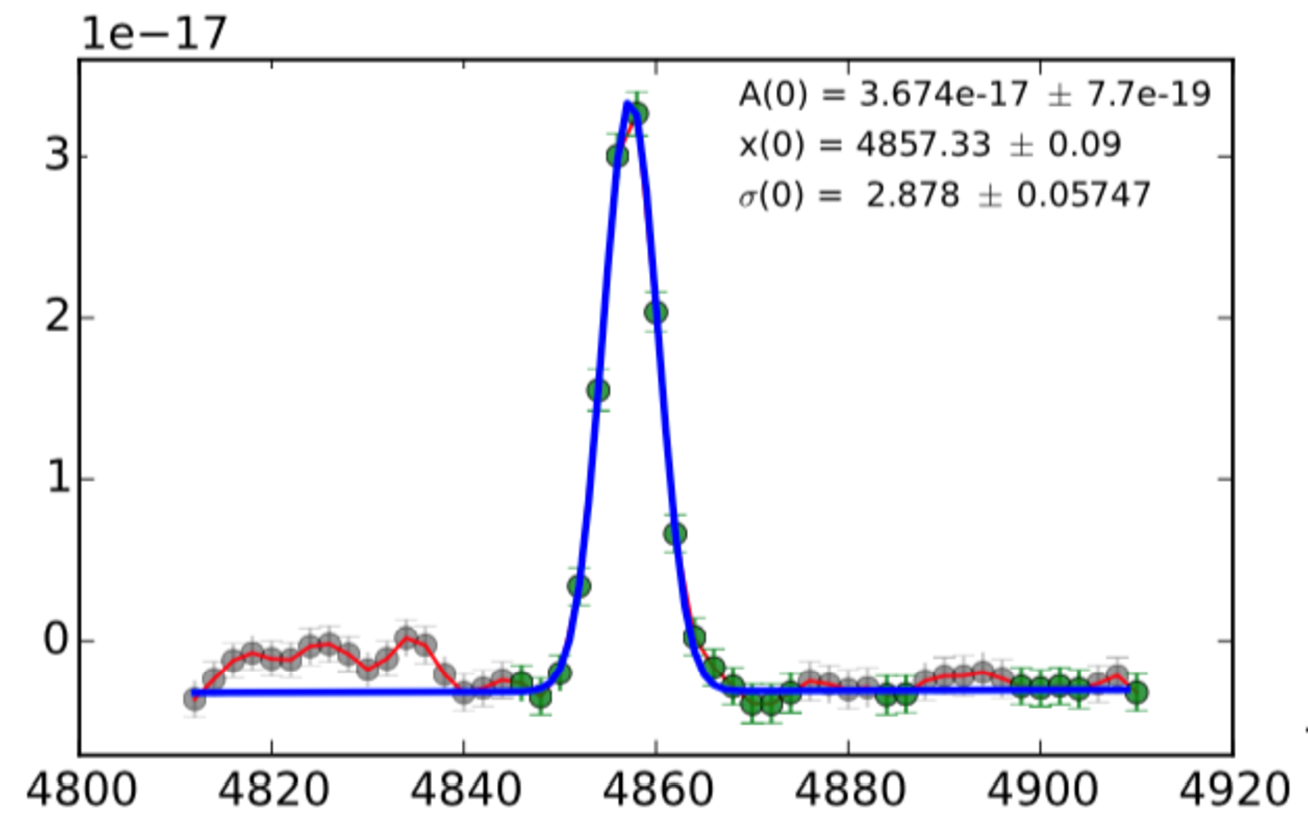
\includegraphics[scale=0.4]{figuras/K0012-zone0-Hb.pdf}
	\caption[Exemplo de ajuste de linha de emissão]
	{Espectro na região da linha de \Hbeta em emissão para a zona central da galáxia UGC00148 (objeto
CALIFA 12) juntamente com o melhor ajuste utilizando uma gaussiana. Em destaque a amplitude (A), o
comprimento de onda central (x) e o desvio padrão neste ajuste (\sigma).}
	\label{fig:rgbline}
\end{figure}
%---------------------------- Figure ----------------------------

%Nem todas as regiões das galáxias que estudamos têm medidas das linhas espectrais necessárias para este estudo. Essa falta não é um defeito de observação e sim uma característica intrínseca de determinada região.
%e nem todas as partes da galáxia possuem gás.
As linhas em emissão geralmente estão ligadas a processos de ionização do gás. O processo de ajuste das linhas de emissão foi feito utilizando o {\sc sherpa} IFU line fitting software (SHIFU; García-Benito et al. em prep.), baseado no pacote {\sc ciao's sherpa} \citep{Freeman.etal.2001, Doe.etal.2007}. Esse programa ajusta perfis gaussianos nas linhas de emissão presentes nos espectros residuais, além de estimar os erros envolvidos neste processo. Em um ajuste normal Gaussiano, os parâmetros geralmente são livres, todavia o ajuste leva em conta uma série de linhas de emissão que estão interligadas, regidas pela física de processos radiativos. Portanto, nessa tarefa alguns parâmetros são interligados e limitados de maneira conjunta. Por exemplo, nos ajustes utilizados neste trabalho as linhas do \nii têm suas {\ATR amplitudes [\ojo ERRADO. FLUXOS AMARRADOS!]} amarradas ($A_{6584}/A_{6548} = 2.9$). Também fixa-se a cinemática das linhas de mesmo íon.

Um exemplo pode ser observado na Fig.\ \ref{fig:rgbline}. Nela vemos a linha de \Hb na zona central do objeto UGC00148 e o ajuste feito pelo programa. Essas medidas podem ser muito sensíveis no caso das linhas serem fracas, como é o caso de \Hb. Nosso estudo usa basicamente o fluxo de \Ha, que é muito menos afetado por incertezas. De fato, a mediana de SN$_{\Ha}$ para todas as zonas é 16 e apenas em 5\% dos casos SN$_{\Ha} < 1$. No Apêndice \ref{apendice:EmLinesDataCube} apresento o programa criado para organizar os resultados dos ajustes das linhas de emissão bem como alguns exemplos de utilização. Com essa classe em mãos, produzi estudos comparativos entre propriedades nebulares e estelares, expostos no Apêndice \ref{apendice:synvsneb}

{\ATR\ojo sugiro engordar com mais uns plots de linhas na fig 2.1. outras linhas, como o3, n2, ha..}

\section{Mapas de exemplo}
\label{sec:sample:maps}
%---------------------------- Figure ----------------------------
\begin{figure}
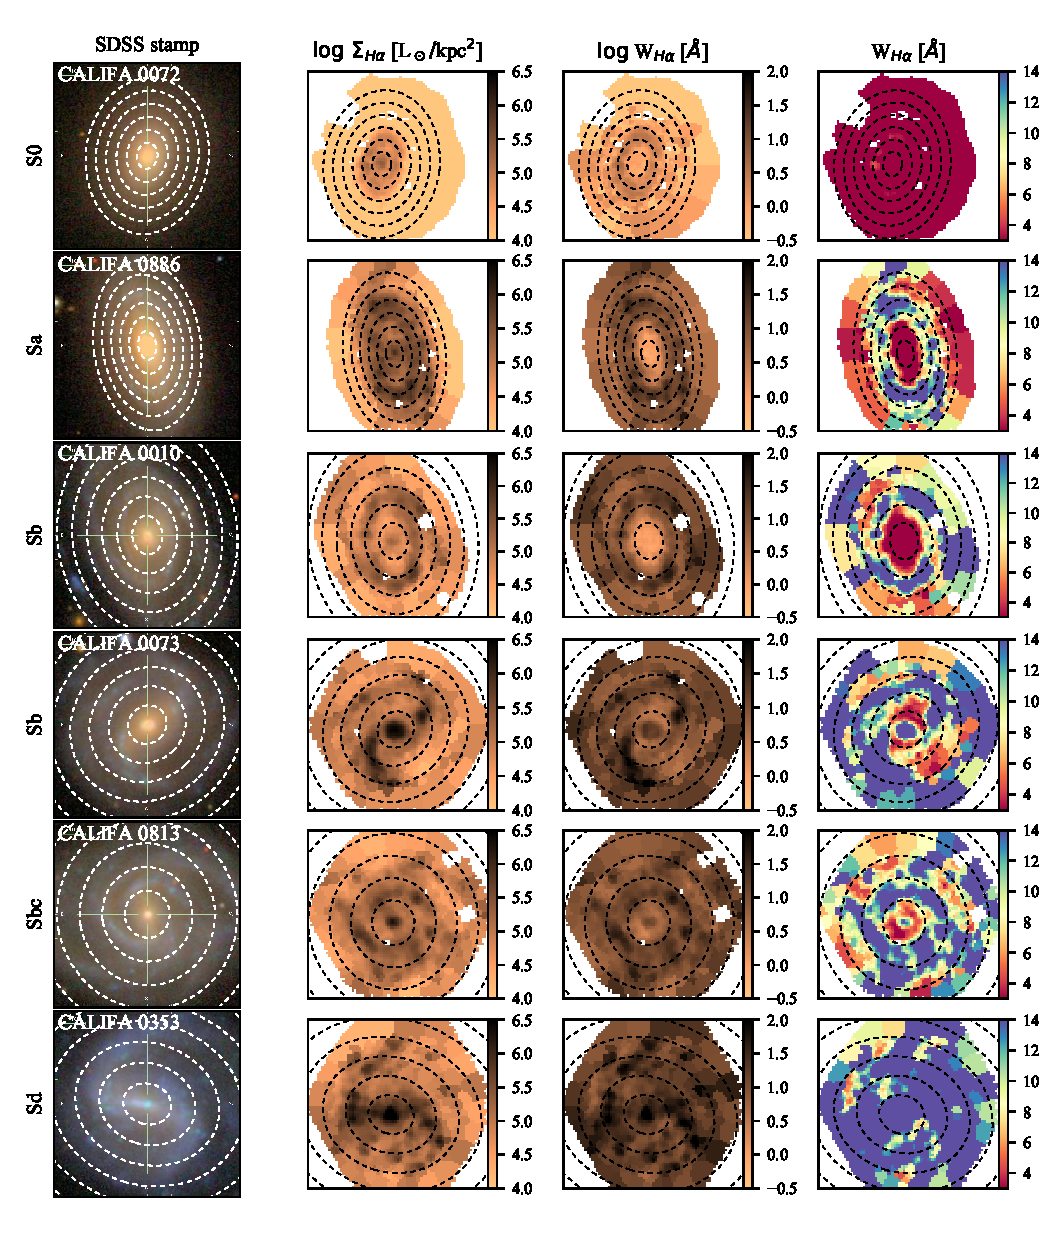
\includegraphics[scale=0.9]{figuras/fig_maps_class_faceon_paper.pdf}
 \caption[Imagem \SDSS e mapas de $\Sigma_{{\rm H}\alpha}$ e $W_{{\rm H}\alpha}$]
 {Imagens do \SDSS e os mapas de $\Sigma_{\Ha}$ e $W_{\Ha}$ para algumas galáxias do CALIFA. Os mapas da coluna mais à direita mostram $W_{\Ha}$ com as cores saturadas em 3 e 14 \AA, evidenciando a classificação proposta para hDIG, mDIG e SFc. Anéis elípticos tracejados demarcam distâncias radiais ao núcleo de $R = 0.5$, 1.0, 1.5, \dots em unidades do raio de meia luz ({\em half-light radius}; HLR). Píxels em branco são fontes externas, como estrelas de campo, ou outros artefatos.}
 \label{fig:ExampleMaps}
\end{figure}
%---------------------------- Figure ----------------------------

Uma seleção de galáxias de nossa amostra com imagem retirada do \SDSS, assim como os mapas de $\Sigma_{\Ha}$ e $W_{\Ha}$ pode ser visto na Figura \ref{fig:ExampleMaps}. Elipses tracejadas marcam até 3 HLR, em passos de 0.5 HLR. Como demonstrado em \citet{Perez.etal.2013}, \citet{Sanchez.etal.2014} e \citet{GonzalezDelgado.etal.2016a}, o HLR é uma boa unidade para comparação entre galáxias de diferentes tamanhos. Para nossa amostra, o HLR = $3.9 \pm 1.7$ kpc (média $\pm$ dispersão). Em galáxias espirais, podemos associar $R > 1$ HLR com o disco e $R < 0.5$ com o bojo. Para sistemas muito inclinados $R$ perde o sentido, porém essa é uma limitação que não afeta nossos resultados.

Nos mapas presentes na Figura \ref{fig:ExampleMaps} podemos notar algumas regiões mais largas. Essas regiões correspondem às zonas de {\em Voronoi}, usadas para garantir a qualidade dos espectros para serem processados pelo \starlight. Como podemos ver essas regiões são proeminentes nas partes externas, menos brilhantes, das galáxias. Porém, até 1 HLR, 97\% dos spaxels possuem SN > 20, portanto nenhuma binagem espacial é feita. Das $309\,958$ zonas em nossa amostra, $274\,534$ (89\%) são formadas de apenas 1 spaxel. As zonas restantes são formadas de 6 spaxels na mediana.

Parte de nossa análise que segue nos próximos capítulos foi baseada na estatística de $W_{\Ha}$ dos espectros de nossa amostra. É certo que o tamanho diferente das zonas introduz alguma distorção em nossos resultados. Seus efeitos serão discutidos mais adiante, porém podemos antecipar que não afetam os resultados principais apresentados nesta tese.


%:::::::::::::::::::::::::::::::::::::::::::::::::::::::::::::::%
%                                                               %
%                          Capítulo 3                           %
%                                                               %
%:::::::::::::::::::::::::::::::::::::::::::::::::::::::::::::::%

%***************************************************************%
%                                                               %
%                          DIG class                            %
%                                                               %
%***************************************************************%

\chapter{Classificação}
\label{sec:DIGclass}

Nosso objetivo neste trabalho é desenvolver uma maneira de caracterizar as regiões de galáxias pelo seu regime de ionização, ou seja, separar regiões SF e DIG, diferenciar componentes do DIG e ir além, servir de legado para futuros trabalhos que possam utilizar essa classificação no estudo do comportamento de diferentes propriedades estelares sob distintas componentes do ISM. Com isso poderemos, através de comparações com os espectros integrados, dar um passo importante na resolução do {\em conumdrum} envolvendo a espectroscopia de uma fibra (ver Seção \ref{sec:intro:partes}). Neste capítulo apresentaremos o processo de classificação e os estudos em que nos embasamos para tal propósito.
% o víes causado pela mistura dessas diferentes componentes nas assinaturas espectrais,

\section{O papel de $W_{H\alpha}$ na classificação das regiões: hDIG, mDIG e SFc}
\label{sec:DIGclass:WHa}

%---------------------------- Figure ----------------------------
\begin{figure}
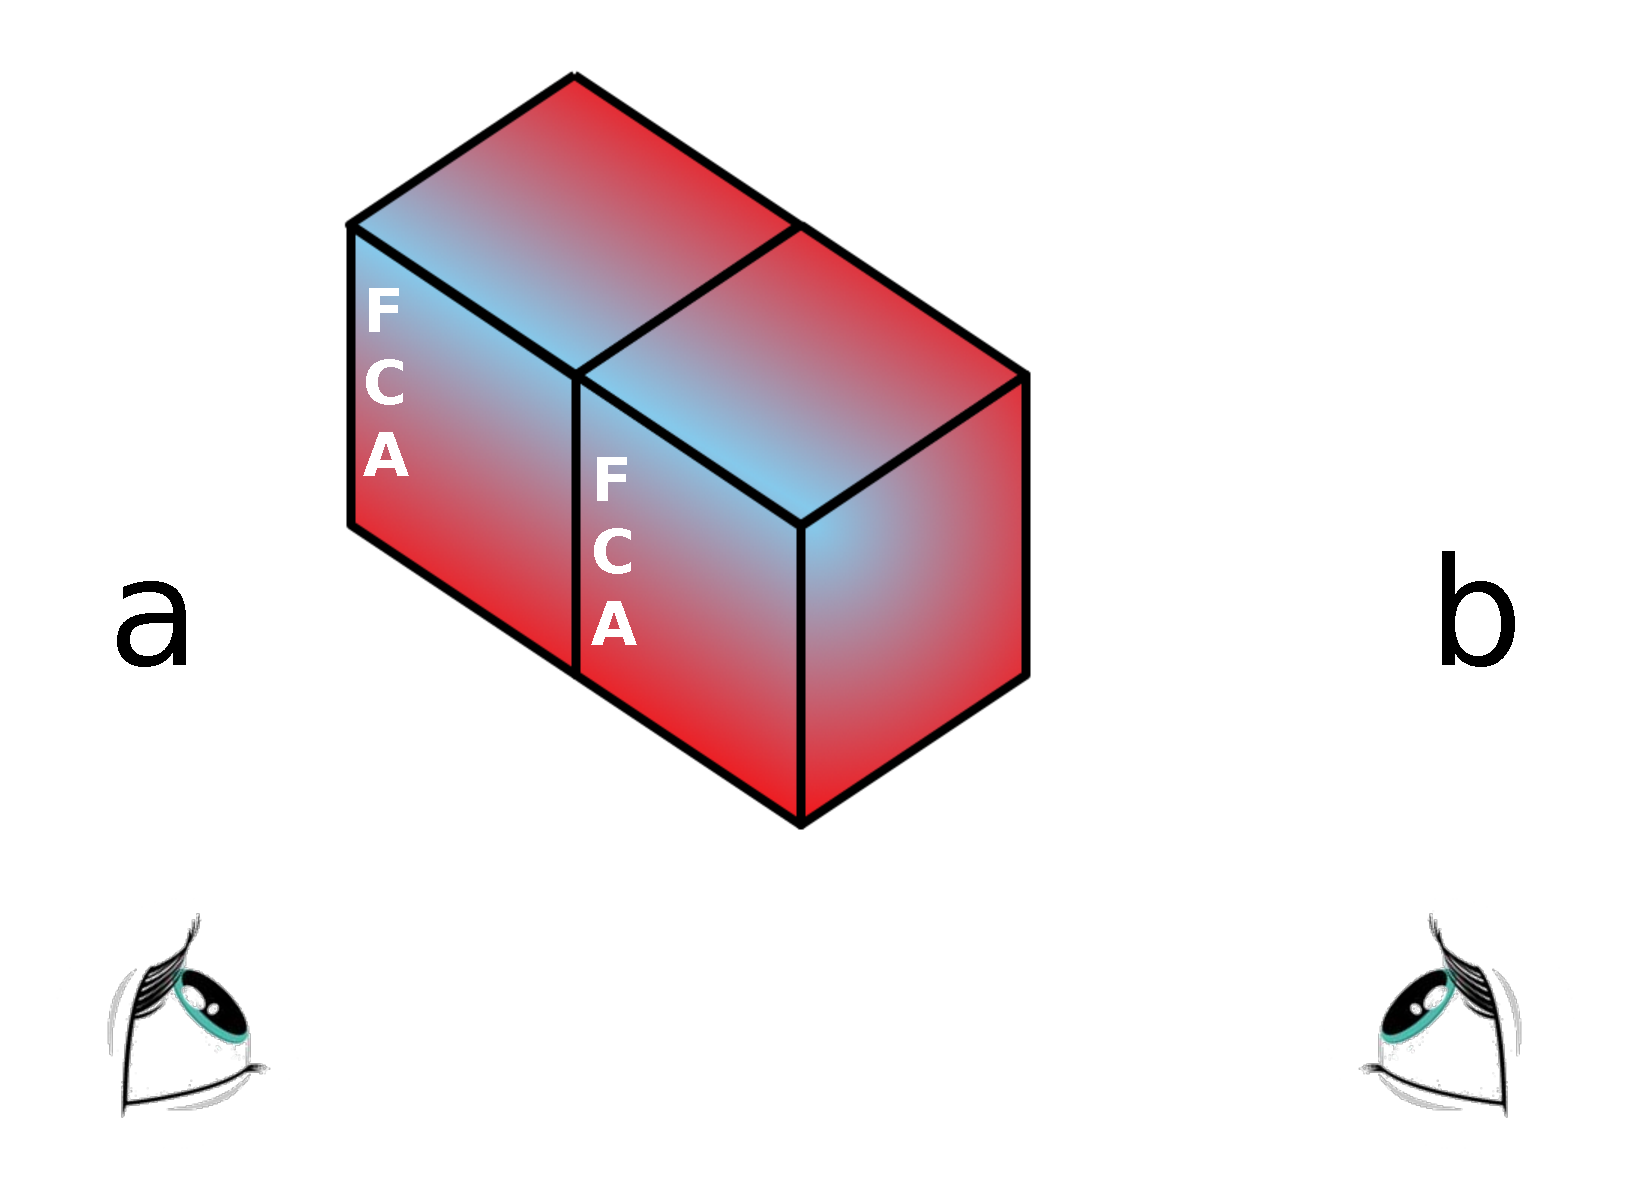
\includegraphics[scale=0.6]{figuras/cubo_com_fundo.pdf}
\caption[Intensive $\times$ extensive]
{A justaposição de dois elementos de volume identicos, emitindo o mesmo fluxo $F$, com a mesma densidade de fluxo $C$ no contínuo, sobre uma área $A$, resulta em uma largura equivalente $W = 2F/2C$. No caso do brilho superficial não, pois temos duas vezes o mesmo fluxo sobre a mesma área quando, $\Sigma = 2F/A$, que é igual a soma dos brilhos individuais. As qualificações `extensivas' e `intensivas' são usadas aqui em analogia à sua conotação termodinâmica: propriedades intensivas são aquelas que não dependem do tamanho ou da massa do sistema (um volume projetado em um {\em spaxel}, como é nosso caso), enquanto que as extensivas são aditivas. Nesse contexto o brilho superficial se comporta como uma propriedade extensiva.}
 \label{fig:intensive_vs_extensive}
\end{figure}
%---------------------------- Figure ----------------------------

Trabalhos anteriores utilizaram o brilho superficial de \Ha na intenção de separar regiões SF e DIG. Por exemplo \citet{Zhang.etal.2017a} argumenta que para os dados do MaNGA, {\em spaxels} onde $\Sigma_{\Ha} > \Sigma_{\Ha}^{\rm SF,min} = 10^{39}$ erg$\,$s$^{-1}\,$kpc$^{-2}$ são confiavelmente dominados por SF.

Como dissemos anteriormente, nós preferimos classificar as regiões entre SF e DIG baseados em $W_{\Ha}$. Vemos na classificação utilizando $\Sigma_{\Ha}$ um erro conceitual que pode ser explicado com um pequeno experimento teórico.

Imagine dois elementos de volume dominados por DIG, ambos com área superficial $A$ emitindo um fluxo $F_{\Ha}=A\times\Sigma_{\Ha}$ como na Figura \ref{fig:intensive_vs_extensive}. Assuma que o meio é opticamente translúcido para os fótons de \Ha (não há extinção), como é apropriado para regiões de DIG, de maneira que o volume inteiro seja visto. Obviamente uma operação de soma com duas regiões DIG não deve alterar a natureza da região observada. Quando vemos uma região ao lado da outra (como no caso `a' na figura), medimos o mesmo brilho superficial, pois temos duas vezes o mesmo fluxo e duas vezes a mesma área, $\Sigma_{\Ha}=(2 \times F_{\Ha})/(2 \times A)$, mantendo uma possível classificação através de um limite no brilho superficial válida. Por outro lado, quando vemos os dois elementos sobrepostos (ambos sobre a mesma linha de visada como no caso `b' na figura) medimos o dobro do brilho superficial, $\Sigma_{\Ha}=(2 \times F_{\Ha})/A$, fazendo com que uma operação DIG+DIG possa resultar em SF, conceitualmente errada.
%Esse viés é conceitualmente errado, pois duas regiões DIG sobrepostas deveriam continuar sendo classificadas como DIG.
Uma classificação utilizando $W_{\Ha}$ não carrega essa inconsistência por construção pois a largura equivalente final é a mesma independente da forma que os elementos são vistos. Como veremos na Seção \ref{sec:DIGdisc:compSBHa}, nos bojos de galáxias, onde há um percurso óptico maior, essa diferença nos critérios de classificação tem particular importância, podendo levar $\Sigma_{\Ha} > \Sigma_{\Ha}^{\rm SF,min}$ mesmo em absência de formação estelar.

De forma independente, podemos argumentar também que propriedades que possuam uma dependência radial, como cor, densidade de massa estelar, quantidade de gás, entre outras, fazem com que uma classificação usando um limite constante não seja apropriada para todas as partes de uma galáxia. Particulamente, quando o regime de ionização do DIG é orquestrado por HOLMES, a razão do número de fótons que podem ionizar \Ha por massa estelar é basicamente constante, gerando $W_{\Ha} \sim 1$ \AA\ independentemente dos fluxos envolvidos (\citealt{Binette.etal.1994a}; \citealt{CidFernandes.etal.2011a}; \citealt{Belfiore.etal.2016} -- ver também a Seção \ref{apendice:EmLinesDataCube:props:SFR} que discute o cálculo da taxa específica de fótons que ionizam H por unidade de massa formada, $q_h$). Dessa forma é fácil entender que, quando o parâmetro é um limite constante em $\Sigma_{\Ha}$, regiões DIG ionizadas por HOLMES (hDIG) com \Ha muito brilhante possam ser erroneamente classificadas como SF. Da mesma forma podemos ter regiões SF fracas classificadas como DIG devido a um baixo $\Sigma_{\Ha}$.



\section{A distribuição observada de $W_{H\alpha}$ e a componente hDIG}
\label{sec:DIGclass:WHaDistrib_hDIG}

%---------------------------- Figure ----------------------------
\begin{figure}
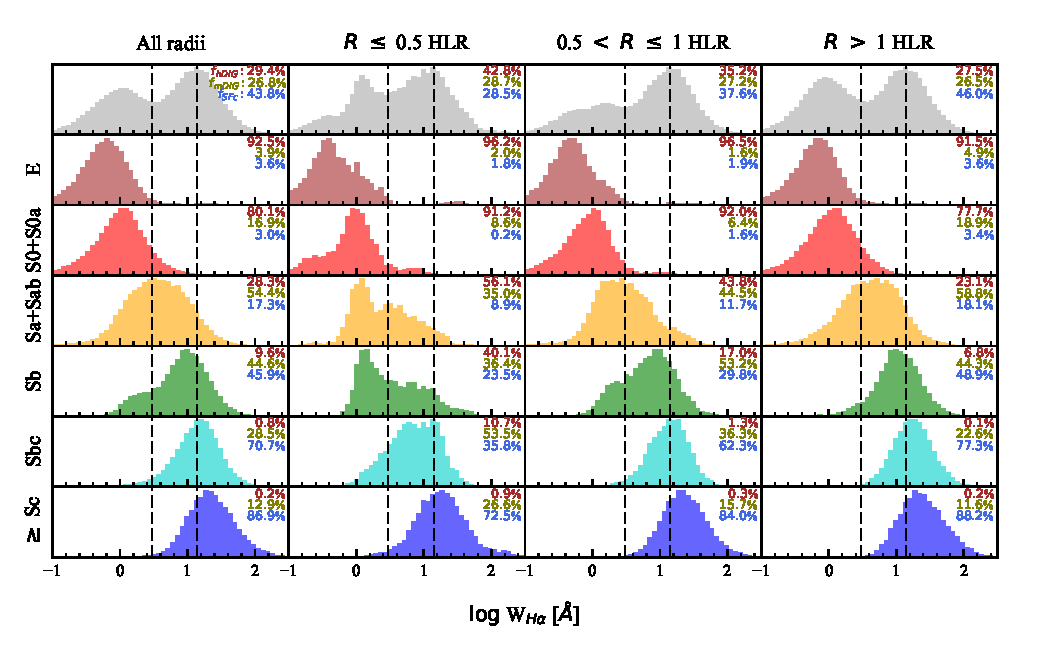
\includegraphics[scale=0.9]{figuras/fig_WHa_histograms_per_morftype_and_radius_cumulFHa.pdf}
\caption[Histogramas de $W_{{\rm H}\alpha}$]
{Distribuição de $W_{\Ha}$ entre $307\,958$ zonas de 391 galáxias do CALIFA. A amostra está segmentada pela classificação de Hubble, de elípticas (segunda linha) até Sc ou mais tardias (última linha). Resultados para a amostra completa estão na primeira linha. Histogramas na primeira coluna identificam regiões de todas as partes das galáxias. Demais colunas selecionam diferentes intervalos em raio: os primeiros 0.5 HLR internos (segunda coluna), $R = 0.5$--1 HLR (terceira) e regiões exteriores com $R > 1$ HLR (quarta). Linhas tracejadas verticais marcam 3 e 14 \AA\,, as divisões entre hDIG/mDIG e mDIG/SFc respectivamente. Os números em cada gráfico representam a fração do fluxo de \Ha associada a cada componente (valor médio entre as zonas das galáxias apresentadas em cada painel).}
 \label{fig:WHaDistrib_ALLgals}
\end{figure}
%---------------------------- Figure ----------------------------

A Figura \ref{fig:WHaDistrib_ALLgals} mostra a distribução observada de $W_{\Ha}$ para $\sim$ 300 mil zonas de 391 galáxias. Na primeira linha temos a amostra inteira e nas linhas seguintes classificamos as zonas conforme a morfologia da galáxia de onde a zona pertence; (6 classes morfológicas: E, S0-S0a, Sa-Sab, Sb, Sbc e $\ge$ Sc). Na primeira coluna temos dados de todas as regiões das galáxias, nas demais colunas classificamos as zonas por intervalos de diferentes raios: $R$ $\le$ 0.5 HLR, 0.5 < $R$ $\le$ 1 HLR, $R$ > 1 HLR.

%---------------------------- Figure ----------------------------
\begin{figure}
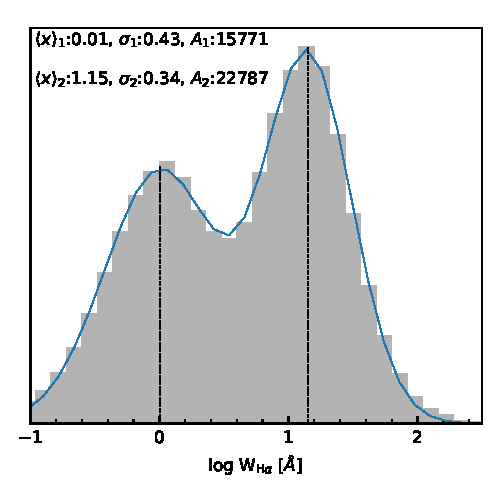
\includegraphics[scale=0.9]{figuras/bimodalWHa_model.pdf}
\caption[Ajuste gaussiano de $W_{\Ha}$]
{Ajuste bimodal de gaussianas com os parâmetros média, desvio padrão e amplitude, índices 1 e 2 representam as duas populações, baixo e alto $W_{\Ha}$ respectivamente entre todas zonas de nossa amostra. As linhas tracejadas verticais são as médias evidenciando os centros de nossas duas populações, 1 e 14 \AA.}
 \label{fig:bimodal_model}
\end{figure}
%---------------------------- Figure ----------------------------

Podemos ver que o histograma com todas as regiões de todas as galáxias (painel topo esquerdo) é claramente bimodal. Distinguimos duas populações com picos em $\sim 1$ \AA\ (baixo $W_{\Ha}$) e $\sim 14$ \AA\ (alto $W_{\Ha}$). Esse comportamento já foi verificado utilizando dados de galáxias do \SDSS \citep{Bamford.etal.2008a, CidFernandes.etal.2011a}. Trabalhos anteriores com dados espacialmente resolvidos do CALIFA \citep{Morisset.etal.2016} e do MaNGA \citep{Belfiore.etal.2016, Belfiore.etal.2017} também identificaram essa bimodalidade.

%Antes de prosseguir, devemos dizer que estudamos também os mesmos histogramas sem a binagem espacial (todos os {\em spaxels}). Como a área é proporcional a $R^2$, o número de {\em spaxels} aumenta quando aumentamos a distância. Devido a prevalencia de regiões de formação estelar nos discos de galáxias espirais ($\ge$ Sb; $R > 1$)
%, maior número presente na nossa amostra,
%Como as regiões presentes nas regiões exteriores de galáxias espirais ($\ge$ Sa), maior número presente na nossa amostra, são dominadas por SF,
%ocorre um aumento na amplitude relativa entre os picos das duas populações, porém a bimodalidade se mantém. Vemos que há um aumento de quase três vezes dessa população, enquando, na população de baixo $W_{\Ha}$, o aumento é de apenas $\sim 20\%$. Como anteriormente, o histograma de todos os dados pode ser ajustado utilizando duas gaussianas, identificando duas componentes com centros em $\sim 1$ e $14$ \AA.

{\ATR \ojo faltou 1 ou 2 frases sobre a fig \ref{fig:bimodal_model} !! Tvz possas botar tb um painel com os histograma e seu ajuste para spaxels (isso q discutes logo abaixo).}

Antes de prosseguir, devemos dizer que estudamos também os mesmos histogramas utilizando os dados sem binagem espacial (todos os {\em spaxels}). Identificamos um aumento na amplitude relativa entre os picos das duas populações, porém a bimodalidade se mantém. Isso ocorre pois a área de uma galáxia é proporcional a $R^2$, assim o número de {\em spaxels} cresce quadráticamente quando aumentamos a distância ao centro. Como vemos na Figura \ref{fig:WHaDistrib_ALLgals}, devido a prevalência de regiões de formação estelar nos discos de galáxias espirais, esse aumento na amplitude relativa é um fenômeno esperado. Observamos um aumento de quase três vezes no número de regiões de alto $W_{\Ha}$ com $R > 1$ HLR nas galáxias Sb e mais tardias, enquanto, na população de baixo $W_{\Ha}$, o aumento é de apenas $\sim 20\%$. Como anteriormente, o histograma de todos os dados pode ser ajustado utilizando duas gaussianas, identificando duas componentes com centros em $\sim 1$ e $14$ \AA.

%, maior número presente na nossa amostra,
%Como as regiões presentes nas regiões exteriores de galáxias espirais ($\ge$ Sa), maior número presente na nossa amostra, são dominadas por SF,
%ocorre

Nossa interpretação é que essa população com baixas larguras equivalentes é formada por regiões DIG fotoionizadas por HOLMES. Como teste, podemos calcular $\xi$, a razão entre a luminosidade de \Ha observada e aquela esperada pelos fótons produzidos pelas populações mais velhas que $10^8$ anos, através da análise com o \starlight, seguindo a metodologia aplicada em \citet{CidFernandes.etal.2011a}. Como os modelos de populações estelares utilizados pela síntese \citep{Gonzalezdelgado2005, Vazdekis2010} não possuem a parte ionizante nos espectros ($h\nu \ge 13.6$ eV) tomamos emprestado aqueles de \citet{Bruzual.Charlot.2003} utilizando uma função inicial de massa ({\em initial mass function}; IMF) de Salpeter e as {\ATR ??\ojo?? trilhas} estelares de \citet{Girardi2000}. Como discutido em \citet{CidFernandes.etal.2011a} distintos modelos produzem diferenças sistematicas de 0.2--0.5 dex na quantidade  prevista de fótons ionizantes. A Figura \ref{fig:WHa-Xi} mostra $\xi$ em função de $W_{\Ha}$, com os histogramas coloridos por nossa classificação hDIG/mDIG/SFc. Verificamos que $\xi$ é de ordem 1 para as regiões com baixo $W_{\Ha}$. Consequentemente, apesar de todas as incertezas envolvidas nesse cálculo \citep{CidFernandes.etal.2011a, Belfiore.etal.2016, Morisset.etal.2016}, o resultado final corrobora a interpretação de que HOLMES são responsáveis pela população de baixo $W_{\Ha}$.


% Seja $L_{\Ha}$ a luminosidade observada de \Ha e $L_{\Ha}^{\rm exp}(t > 10^8 {\rm anos})$ a luminosidade esperada pelas populações velhas, definimos a razão como:
% \begin{equation}
%   \xi\ =\ \frac{L_{\Ha}}{L_{\Ha}^{\rm exp}(t > 10^8 {\rm anos})}.
% \end{equation}
% \noindent Podemos definir

%---------------------------- Figure ----------------------------
\begin{figure}
 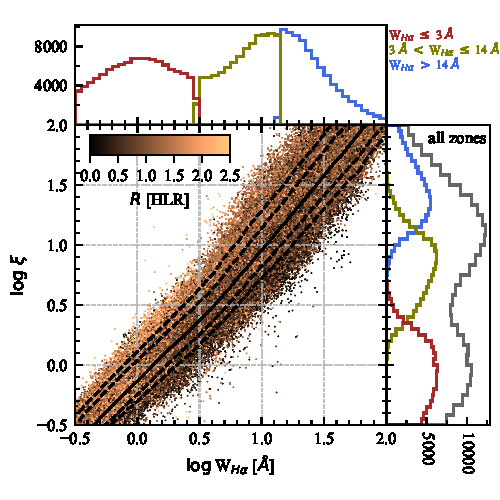
\includegraphics[scale=1.5]{figuras/fig_logxi_logWHa_histograms.pdf}
 \caption[$\log \xi \times \log {\rm H}\alpha$]
 {Razão entre a luminosidade de \Ha observada e aquela predita pelas poulações mais velhas que $10^8$ anos ($\xi$) em função de $W_{\Ha}$ para todas as zonas de nossa amostra. Os pontos estão coloridos conforme a distânciada até o núcleo (em unidades de HLR). Os histogramas de $\xi$ e de $W_{\Ha}$ estão coloridos como vermelho/amarelo/azul (hDIG/mDIG/SFc), mostrando que as regiões com baixo $W_{\Ha}$ são compatíveis com ionização por HOLMES.}
 \label{fig:WHa-Xi}
\end{figure}
%---------------------------- Figure ----------------------------

Fica evidente a correspondência dessa interpretação com o conceito de galáxias aposentadas apresentado por \citet{Stasinska.etal.2008a}. Estes são sistemas que pararam de formar estrelas há muito tempo, nos quais os fótons ionizantes presentes são provenientes das estrelas que já evoluíram após o ramo assintótico das gigantes ({\em post-asymptotic giant branch; post-AGB}) e de anãs brancas, levando os valores de $W_{\Ha}$ a $\sim 1$ \AA. O limite de 3 \AA\ que cinge essa população coincide com o valor utilizado por \citet{CidFernandes.etal.2011a} para distinguir galáxias aposentadas daquelas com regime de ionização dominado por SF ou por AGN. Por esse motivo nós \ED{sugerimos fortemente} \ED{\sout{firmemente indicamos}}
que as populações com $W_{\Ha} < 3$ \AA\ sejam classificadas como gás ionizado difuso por HOLMES, o hDIG.

A separação da distribuição de $W_{\Ha}$ por tipos de Hubble mostra que a bimodalidade está sempre presente, mudando apenas a proporção entre as populações de baixo e alto $W_{\Ha}$ conforme a morfologia: galáxias {\em early-type} são esmagadoramente dominadas por valores ao redor do pico de $\sim 1$ \AA, enquanto nas galáxias espirais tardias é a população com alto $W_{\Ha}$ que domina.

Quando dividimos a amostra em intervalos de $R$ vemos que a população hDIG se distribui igualmente entre as galáxias {\em early-type}, confirmando estudos anteriores de \citet{Kehrig.etal.2012}, \citet{Singh.etal.2013}, e \citet{Gomes.etal.2016b}, além das análises baseadas em dados do MaNGA por \citet{Belfiore.etal.2016, Belfiore.etal.2017}. Entre as Sb e espirais mais tardias o hDIG fica concentrado nas regiões centrais das galáxias. Colocando isso em números, 82\% dos pontos hDIG das 225 galáxias Sb ou mais tardias estão localizados em regiões onde $R < 1$ HLR.

Nós interpretamos essa alta incidência de zonas hDIG nas regiões centrais como um corolário da prevalência de populações velhas nos bojos.
Qualquer outro tipo de fonte de ionização relevante
além de HOLMES
elevaria os valores de $W_{\Ha}$. Por outro lado, a baixa incidência de regiões com $W_{\Ha} < 3$ \AA\ situadas a grandes distâncias do centro ($R$ grande) em galáxias espirais indica que a emissão hDIG não é estatisticamente relevante para o DIG que permeia as regiões SF presentes em seus discos. A Figura \ref{fig:WHaDistrib_ALLgals} também mostra que apesar do hDIG explicar uma parte substancial da emissão nos discos de galáxias Sa--Sab, entre as Sb ou mais tardias \ED{são raros os discos dominados por hDIG.} \ED{\sout{são raras as incidências de discos dominados pelo hDIG.}}

Podemos ver que a introdução da categoria hDIG em nossa classificação é eregida sob um cenário criado por argumentos teóricos e experimentais. Essa componente do DIG está muito bem compreendida e se torna dominante sempre que HOLMES são a fonte de ionização mais relevante.

Finalizamos esta seção analisando a extensão que efeitos de inclinação podem causar na distribuição de $W_{\Ha}$. Para esse experimento primeiro eliminamos galáxias elípticas (E e S0) de nossa amostra. Então dividimos a amostra por classes de diferentes $b/a$ (elipticidade\footnote{a razão entre o eixo maior e o eixo menor de uma elipse}, conforme cálculo detalhado em \citealt{deAmorim.etal.2017}). O único efeito digno de nota é que
\ED{\sout{ao observarmos zonas com $R < 0.5$ HLR existe um efeito de projeção. Ao irmos de galáxias {\em edge-on} para {\em face-on}, os histogramas tendem a se deslocarem $\sim$ 0.2--0.3 dex {\ATR na direção de valores mais baixos de $W_{\Ha}$}}}.
%[\ojo NAO FAZ SENTIDO / EH O CONTRARIO DO QUE ABAIXO EXPLICAS!!!]}}}
\ED{nas zonas mais internas ($R < 0.5$ HLR) notamos um efeito de projeção, no qual ao irmos de galáxias {\em face-on} para {\em edge-on}, essas regiões tendem para valores $\sim$ 0.2--0.3 dex na direção de valores mais altos de $W_{\Ha}$.} Isso acontece pois enquanto regiões centrais em galáxias {\em face-on} amostram o bojo, que tem características hDIG, ao aumentarmos a inclinação \ED{(indo na direção das galáxias {\em edge-on}),} partes do disco ficam projetadas sob a linha de visada, resultando numa mistura de regiões SFc e hDIG. Porém, assim como os efeitos da binagem espacial usando zonas de Voronoi, os efeitos de inclinação também não apagam a dicotomia fundamental entre esses dois regimes nebulares.

\edu{Cid, pelo que eu entendo isso está correto, porém, estava apenas na ordem contrária do que eu explicava abaixo.}

\subsection{Identificação das componentes hDIG, mDIG e SFc}
\label{sec:DIGclass:identclass}

As populações de baixo $W_{\Ha}$ podem ser seguramente classificadas como hDIG. Diferentemente, as populações de alto $W_{\Ha}$ não podem ser identificadas univocamente como de tipo SF. Certamente as regiões SF estão entre essas com $W_{\Ha}$ \ED{$ > 3$ \AA}, porém outros processos de ionização \ED{\sout{podem guiar a disponibilidade de fótons ionizantes dessas regiões}} \ED{estão incluídos nessa população.}
%{\ATR guiar a disponibilidade de fótons ionizantes dessas regiões [\ojo ??que?? reword]}.
Em particular, a ionização do DIG por fótons que escapam de regiões \hii está entre esses processos. Nesse caso, a razão de fótons ionizantes por unidade de massa estelar eleva os valores de $W_{\Ha}$ acima daqueles típicos em regiões ionizadas por HOLMES.

Sabendo que a população com alto $W_{\Ha}$ representa uma mistura de regimes, é útil subdividi-la entre mDIG e SFc, de maneira a identificar zonas onde a formação estelar é a fonte de ionização relativamente mais importante. Não existe fronteira conspícua que possa diferenciar regiões SFc de mDIG em função de $W_{\Ha}$. Como podemos ver na Figura \ref{fig:WHaDistrib_ALLgals}, a população com alto $W_{\Ha}$ é unimodal, não sugerindo a existência de subpopulações e sim de uma distribuição contínua. Na falta de um valor que possa ser usado como critério para a divisão entre mDIG e SFc utilizamos 14 \AA\ para tal classificação, coincidindo com o pico da distribuição dessa população
(Figura \ref{fig:bimodal_model}).

Nosso esquema final de classificação é, portanto:

\begin{itemize}
 \item hDIG: $W_{\Ha} \le 3 \,\mathrm{\AA}$,
 \item mDIG:  $3 \,\mathrm{\AA}  < W_{\Ha} \le 14 \,\mathrm{\AA}$,
 \item SFc: $W_{\Ha} > 14 \,\mathrm{\AA}$.
\end{itemize}

Devemos levar em conta uma assimetria conceitual nessa classificação. Enquanto a fronteira hDIG/mDIG em 3 \AA\ é firmemente ancorada em um conhecimento teórico da natureza da população hDIG, totalmente corroborada pela bimodalidade na distribuição de $W_{\Ha}$, nada nesse nível pode ser afirmado sobre a divisão entre mDIG/SFc. Tudo o que podemos dizer é que regiões com $W_{\Ha}$ acima de 14 \AA\ possuem uma maior proporção de SFc do que aquelas abaixo. Portanto, através dessa classificação, devemos considerar que as regiões mDIG podem carregar alguma formação estelar e que regiões SFc não isolam regiões SF puras. Regiões \hii gigantes genuínas, objetos base para qualquer estudo de linhas de emissão em galáxias, possuem $W_{\Ha}$ uma ordem de grandeza maior \citep{McCall.etal.1985, Garnett.and.Shields.1987, Kennicutt.and.Garnett.1996, Luridiana.and.Peimbert.2001, Bresolin.etal.2004}, porém, como mencionado anteriormente, com a resolução de nossos dados, objetos como esses estão muito diluídos.

Com nossas regiões classificadas podemos retornar ao painel mais à esquerda da Figura \ref{fig:ExampleMaps}. Nele vemos os mapas de $W_{\Ha}$ saturados pelos intervalos $< 3$ \AA\ (hDIG, vermelho) e $> 14$ \AA\ (SFc, azul). Cores intermediárias representam o intervalo de 3--14 \AA\ (mDIG). A galáxia S0 no topo da figura exemplifica o domínio do hDIG sobre as galáxias {\em early-type} como foi previamente inferido dos histogramas de $W_{\Ha}$ na Figura \ref{fig:WHaDistrib_ALLgals}. Através dos mapas das galáxias CALIFA 0886 (NGC 7311) e  0010 (NGC 0036) observamos o domínio da componente hDIG nos bojos de galáxias. Como era esperado, a componente SFc se torna cada vez mais importante a medida que avançamos para tipos mais tardios na classificação de Hubble (seguindo de cima para baixo nas Figuras \ref{fig:ExampleMaps} e \ref{fig:WHaDistrib_ALLgals}).

%%%%%%%%%%%%%%%%%%%%%%%%%%%%%%%%%%%%%%%%%%%%%%%%%%%%%%%%%%%%%%%%%
% Lacerda@CórregoGrande - Jan/2018                              %
%%%%%%%%%%%%%%%%%%%%%%%%%%%%%%%%%%%%%%%%%%%%%%%%%%%%%%%%%%%%%%%%%

%:::::::::::::::::::::::::::::::::::::::::::::::::::::::::::::::%
%                                                               %
%                          Capítulo 4                           %
%                                                               %
%:::::::::::::::::::::::::::::::::::::::::::::::::::::::::::::::%

%***************************************************************%
%                                                               %
%                        DIG discussion                         %
%                                                               %
%***************************************************************%

\chapter{Discussão}
\label{sec:DIGdisc}

%{\ATR Nosso método de classificação é inspirado em argumentos teóricos e empíricos possui diversos propósitos [\ojo reler... a frase nao faz sentido!]}.
\ED{Nosso método de classificação, inspirado em argumentos teóricos e empíricos, possui diversos propósitos}. Neste capítulo vamos aplicar nosso método para nossa amostra do CALIFA com os seguintes objetivos específicos:
\begin{enumerate*}[label=(\roman*)]
    \item estimar a relevância do hDIG, mDIG e SFc sobre galáxias ao longo de toda a sequência de Hubble;
    \item estudar a natureza da emissão difusa extraplanar nos sistemas {\em edge-on};
    \item comparar resultados obtidos com o nosso método frente àqueles que separam SF/DIG baseados em um limite fixo em $\Sigma_{\Ha}$;
    \item investigar a possibilidade de discernimento entre regimes DIG e SF baseados em razões de linhas sensíveis à densidade do meio;
    \item testar a consistência de nosso sistema de classificação analisando através de um diagrama clássico de linhas de emissão;
    \item examinar a mistura presente no mDIG.
\end{enumerate*}
Fechamos esse capítulo com uma discussão sobre os possíveis {\em caveats} em nosso estudo.

\section{A relevância das componentes hDIG, mDIG e SFc}
\label{sec:DIGdisc:relstrenghts}

%---------------------------- Figure ----------------------------
\begin{figure}
 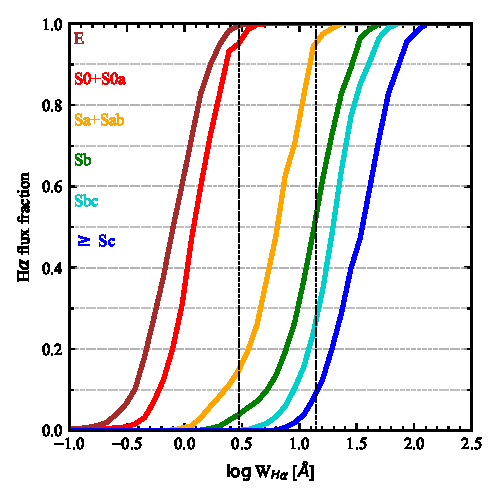
\includegraphics{figuras/fig_cumul_fHaWHa_per_morftype.pdf}
 \caption[Fração cumulativa do fluxo de ${\rm H}\alpha$ com o crescimento de $W_{{\rm H}\alpha}$ para diferentes classes morfológicas]
 {Fração cumulativa do fluxo total de \Ha provenientes de regiões com $W_{\Ha}$ menor que determinado valor. O gráfico mostra as curvas medianas obtidas para galáxias presentes em cada uma de nossas seis classes morfológicas.}
 \label{fig:CurveOfGrowth}
\end{figure}
%---------------------------- Figure ----------------------------

Dentre as questões que podemos perscrutar neste estudo, a importância relativa das componentes de nossa classificação talvez seja a mais importante. A dominância e a evolução da influência que cada um dessas componentes tem sobre galáxias através de diferentes tipos morfológicos é importante na interpretação de propriedades derivadas de dados espectrais não resolvidos espacialmente. Nesses estudos as assinaturas de regimes distintos vêm todas misturadas sob o mesmo espectro.

Uma maneira simples e relevante observacionalmente de quantificar isso é calculando a contribuição relativa de cada componente para o fluxo total de \Ha. Por exemplo, nas galáxias na Figura \ref{fig:ExampleMaps} essas frações percentuais vão de $(f_{\rm hDIG} , f_{\rm mDIG} , f_{\rm SFc}) = (87,13,0)$ para a galáxia S0 CALIFA 0072, até $(5.5,47,47.5)$ para a galáxias Sb CALIFA 0010, e $(0.3,46.1,53.6)$ para a CALIFA 0813, uma Sbc. Essa progressão ao longo da sequência de Hubble reflete as tendências que podem ser vistas na Figura \ref{fig:WHaDistrib_ALLgals}. No canto superior direito de cada painel temos os valores de $(f_{\rm hDIG} , f_{\rm mDIG} , f_{\rm SFc})$ para diferentes distâncias radiais e diferentes tipos morfológicos.

De maneira mais elaborada, a Figura \ref{fig:CurveOfGrowth} mostra essas frações para toda a amostra através dos valores medianos de cada classe morfológica. Nós calculamos a fração cumulativa do fluxo de \Ha, $f$, proveniente de regiões que possuem $W_{\Ha}$ menor que determinado valor. As curvas de $f(<W_{\Ha})$ representam como a fração cumulativa cresce com relação a $W_{\Ha}$. Na figura mostramos as curvas medianas para as nossas seis classes morfológicas. As linhas tracejadas verticais representam nossas fronteiras hDIG/mDIG e mDIG/SFc, em 3 e 14 \AA\ respectivamente.

A progressão constante de {\em early-} para {\em late-type} nessas curvas confirmam nossas expectativas provenientes das distribuições de $W_{\Ha}$ (Figura \ref{fig:WHaDistrib_ALLgals}) além de também nos permitir quantificar a importância relativa entre as componentes e o fluxo total de \Ha. Em galáxias elípticas ou S0 temos praticamente toda a emissão de \Ha na fase hDIG ($W_{\Ha} \le 3$). Entre os sistemas Sa-Sab, essa componente se encarrega por 14\% do fluxo de \Ha, com o mDIG sendo o responsável por praticamente todo o fluxo restante. De Sb para frente, o regime SFc domina, sendo responsável por 50\% ou mais.
%Naturalmente existe um espalhamento natural nos dados, mesmo quando divididos em classes morfológicas.

A contribuição relativa do DIG para a emissão em \Ha foi estimada em diversos estudos anteriores, geralmente baseados em dados obtidos com filtros estreitos (\Ha + \nii) \citep{Ferguson.etal.1996, Zurita.etal.2000, Thilker.etal.2002, Oey.etal.2007}, com resultados variando substancialmente principalmente devido a diferenças na metodologia de separação da emissão difusa. O maior estudo até hoje foi feito por \citet{Oey.etal.2007}, que estimaram a fração de emissão difusa em \Ha de $59\pm19 \%$ sobre uma amostra de 109 galáxias do {\em survey} SINGG \citep{Meurer.etal.2006}. Para nossa amostra (e nossas definições) nós encontramos um valor bem próximo, 56\% (hDIG + mDIG), mas com um espalhamento muito maior, $\pm38 \%$. Diferentemente de nosso estudo (Figura \ref{fig:CurveOfGrowth}), eles não encontraram nenhuma evidencia de correlação com o tipo morfológico. Talvez o motivo seja devido a diferença de critério e metodologia de classificação DIG/SF.


\section{Emissão extraplanar em sistemas {\em edge-on}}
\label{sec:DIGdisc:edgeon}

%---------------------------- Figure ----------------------------
\begin{figure}
 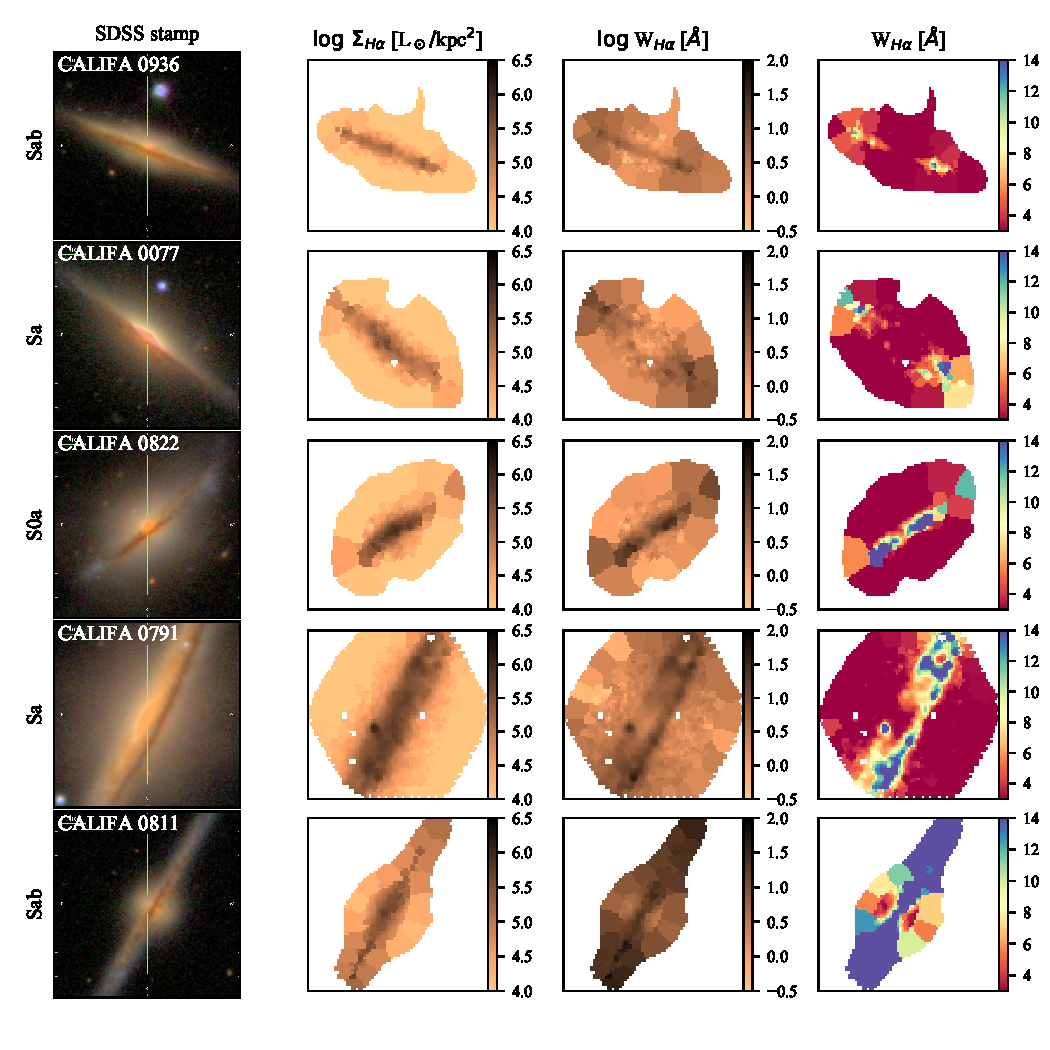
\includegraphics{figuras/fig_maps_class_edgeon_paper.pdf}
 \caption[Imagem \SDSS e mapas de $\Sigma_{{\rm H}\alpha}$ e $W_{{\rm H}\alpha}$: sistemas {\em edge-on}]
 {Como a Figura.\ \ref{fig:ExampleMaps}, mas para galáxias {\em edge-on}.}
 \label{fig:ExampleMapsEdgeOn}
\end{figure}
%---------------------------- Figure ----------------------------

%Devido ao comportamento sistemático das propriedades de linhas de emissão, esses
Sistemas altamente inclinados são importantes para o estudo da emissão DIG nas regiões acima (e abaixo) do disco galáctico \citep{Tullmann.and.Dettmar.2000, Otte.etal.2002, Jones.etal.2017}. A galáxia protótipo utilizada nesses estudos é a NGC 891, extensivamente observada em diversos comprimentos de onda \citep{Rand.1998, Hodges.and.Bregman.2013, Seon.etal.2014, Hughes.etal.2015}. Esses estudos enfatizaram que as propriedades de linhas de emissão observadas no DIG extraplanar não podem ser explicadas puramente por fótons ionizantes que escapam de regiões \hii presentes no disco. Uma variedade de fenômenos que podem  gerar tal emissão foram sugeridos, como: dissipação de turbulência \citep{Minter.and.Spangler.1997}, reconexão magnética \citep{Raymond.1992}, choques \citep{CollinsRand.2001}, raios cósmicos, aquecimento fotoelétrico proveniente de grãos de poeira do meio interestelar  \citep{Weingartner.and.Draine.2001}, e fótons do contínuo de Lyman vindos de estrelas velhas e quentes \citep{FloresFajardo.etal.2011a}.

A Figura \ref{fig:ExampleMapsEdgeOn}  mostra como os dados do CALIFA podem nos trazer um novo {\em insight} ao problema. Nela vemos cinco exemplos de galáxias {\em edge-on} dispostas da mesma forma que na Figura \ref{fig:ExampleMaps}. As quatro primeiras galáxias possuem configuração muito parecida, onde temos o disco e arredores dominados por mDIG e SFc, enquanto a grandes distâncias do disco galácticos vemos uma completo predomínio de hDIG. Isso favorece o cenário proposto por \citet{FloresFajardo.etal.2011a}, onde a ionização se torna dominada por HOLMES à medida que nos afastamos do plano galáctico. Essa conclusão é reforçada pelos mapas de diagnóstico de razões de linhas baseados em dados do MaNGA em \citet{Belfiore.etal.2016} e \citet{Zhang.etal.2017a}.

Através de nossa experiência calculando $\xi$ (veja a Seção \ref{sec:DIGclass:WHaDistrib_hDIG}) podemos, pela primeira vez, relacionar a emissão DIG extraplanar com as populações estelares subjacentes. A mediana de $\xi$ nas regiões extraplanares das quatro primeiras galáxias na Figura \ref{fig:ExampleMapsEdgeOn} é 1.5 com interquartis 1.1--1.9. Dado um fator de incerteza de  $\sim \times ~2$--3 nessa estimativa \citep{CidFernandes.etal.2011a} a conclusão principal aqui é que $\xi$ é da ordem de 1 e por isso consegue produzir fótons com $h\nu > 13.6$ suficientes para explicar a emissão extraplanar de \Ha.

Se essas galáxias fossem vistas {\em face-on}, o DIG extraplanar estaria projetado por cima do disco, que é dominado por mDIG + SFc. Para uma emissividade constante de \Ha, a razão entre $\Sigma_{\Ha}$ {\em face-on} e {\em edge-on} é igual a razão entre $h/r$ (altura e raio) da camada hDIG extraplanar. Nas galáxias da Figura \ref{fig:ExampleMapsEdgeOn} o valor de $\Sigma_{\Ha}$ é de aproximadamente algumas vezes $10^4 L_\odot\,$kpc$^{-2}$. Para $h \sim r$, este também deve ser o brilho superficial dessa componente. Esse valor é muito menor que os que estão presentes nas regiões SFc das galáxias {\em face-on} da Figura \ref{fig:ExampleMaps}, nesse caso, portanto, o efeito do hDIG extraplanar projetado pode ser negligenciado. Porém, algumas regiões mDIG apresentam valores não muito maiores que $10^4 L_\odot\,$kpc$^{-2}$ podendo assim carregar alguma contribuição não-negligenciável do hDIG extraplanar.

A galáxia na última linha da Figura \ref{fig:ExampleMapsEdgeOn} (CALIFA 0811, UGC 10043) é diferente das demais, como podemos ver pelo seu mapa de classificação. Ela possui muito mais SFc no seu disco e em regiões extraplanares, além de um cone bipolar com valores intermediários de $W_{\Ha}$ centrado no núcleo. Essa galáxia foi recentemente estudada por \citet{LopezCoba.etal.2017}, no qual encontraram razões entre linhas de emissão e cinemática consistentes com vento galáctico alimentado por um evento SF central. Essa combinação de ionização por choque e formação estelar espalhada pelo disco explica porque não há emissão hDIG extraplanar nessa galáxia, embora seja curioso que os valores de $W_{\Ha}$ caiam para valores hDIG nas partes internas do bicone.


\section{Comparações com esquemas de separação SF/DIG baseados em $\Sigma_{{\rm H}\alpha}$}
\label{sec:DIGdisc:compSBHa}

%---------------------------- Figure ----------------------------
\begin{figure}
 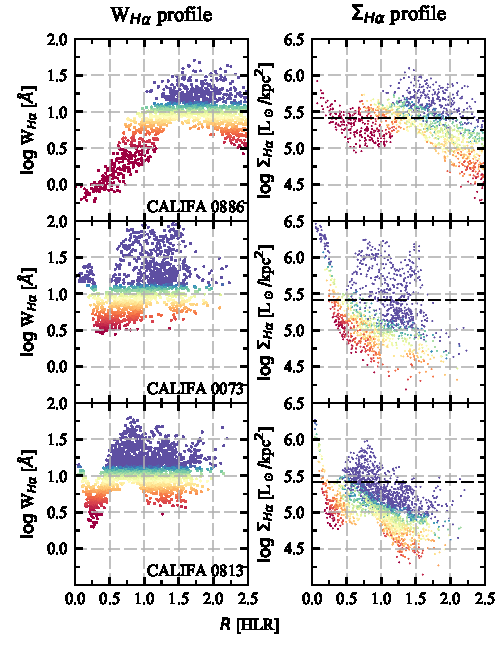
\includegraphics[scale=1.7]{figuras/fig_WHaSBHa_profile_faceon_paper.pdf}
 \caption[Perfis radiais de $W_{{\rm H}\alpha}$ e $\Sigma_{{\rm H}\alpha}$]
 {Perfis radiais de $W_{{\rm H}\alpha}$ e $\Sigma_{{\rm H}\alpha}$ para três galáxias presentes na Figura \ref{fig:ExampleMaps}. Os pontos são coloridos segundo $W_{\Ha}$. As linhas pontilhadas nos painéis da direita marcam $\Sigma_{\Ha} = 10^{39}$ erg$\,$s$^{-1}\,$kpc$^{-2}$.}
 \label{fig:WHa_and_SHa_profiles}
\end{figure}
%---------------------------- Figure ----------------------------

Apesar das vantagens conceituais desse modo de classificação apresentado até agora, $W_{\Ha}$ possui $\Sigma_{\Ha}$ no seu numerador, de modo que pode-se imaginar que um modelo de classificação baseado nessas duas variáveis deveriam ter resultados semelhantes. Através dos mapas da Figura \ref{fig:ExampleMaps} podemos perceber que algumas estruturas, como os braços de formação estelar, são concomitantemente identificados por $W_{\Ha}$ e $\Sigma_{\Ha}$, porém outras não são. Mais precisamente, $\Sigma_{\Ha}$ sempre tem um máximo no centro da galáxia,
%porém para galáxias {\em early-type}, $W_{\Ha}$ mostra evidentes {\ATR declives [\ojo ????QUE??]}.
\ED{contudo, em galáxias {\em early-type}, os valores de $W_{\Ha}$ sempre diminuem quando vamos às partes centrais.}

\ED{A Figura \ref{fig:WHa_and_SHa_profiles} examina esse problema utilizando perfis radiais de três das galáxias presentes na Figura \ref{fig:ExampleMaps}, CALIFA 0886, 0073 e 0813. (Mais exemplos de perfis radiais de $W_{\Ha}$ podem ser encontrados em \citealt{Papaderos.etal.2013, Belfiore.etal.2016, Belfiore.etal.2017, Gomes.etal.2016b, GonzalezDelgado.etal.2016a}.) Na coluna da esquerda (direita) temos os valores de $W_{\Ha}$ ($\Sigma_{\Ha}$) contra R. Ambos são coloridos por $W_{\Ha}$ segundo o mesmo esquema de cores utilizado até aqui.}

%{\ATR [reler e traduzir melhor!!] Três exemplos de galáxias presentes} na Figura \ref{fig:ExampleMaps}, CALIFA 0886, 0073 e 0813, com seus respectivos perfis radiais de $W_{\Ha}$ e $\Sigma_{\Ha}$ aparecem na Figura \ref{fig:WHa_and_SHa_profiles}. (Exemplos de perfis radiais como esses podem ser encontrados em \citealt{Papaderos.etal.2013, Belfiore.etal.2016, Belfiore.etal.2017, Gomes.etal.2016b, GonzalezDelgado.etal.2016a}.) Na coluna da esquerda (direita) temos os valores de $W_{\Ha}$ ($\Sigma_{\Ha}$) contra R. Ambos são coloridos por $W_{\Ha}$ segundo o mesmo esquema de cores utilizado até aqui.

A CALIFA 0886 é um bom exemplo de galáxia que apresenta valores baixos de $W_{\Ha}$ em seu centro dominado por emissão hDIG, porém com um pico em $\Sigma_{\Ha}$ nessa mesma região. A alta concentração de HOLMES no bojo da galáxia faz com que o mesmo seja muito mais brilhante que o disco que o \ED{envolve/cerca} \ED{\sout{cinge}}. O aumento do brilho superficial de \Ha devido a geometria do bojo pode fazer com que essa emissão seja incorretamente classificada como SF quando utilizamos um esquema de classificação SF/DIG baseado em $\Sigma_{\Ha}$. Como vemos no painel do topo à direita, os valores de $\Sigma_{\Ha}$ estão acima da linha pontilhada, que marca o limite que seleciona confiávelmente spaxels dominados por regiões \hii segundo \citet{Zhang.etal.2017a}, $\Sigma^{\rm SF,min}_{\Ha} = 10^{39}$ erg$\,$s$^{-1}\,$kpc$^{-2} =  2.6 \times 10^{5} L_\odot\,$kpc$^{-2}$. No entanto, vemos que as mesmas regiões possuem $W_{\Ha} \sim 1$ \AA, sem dúvidas operando sob regime hDIG. O critério utilizando $W_{\Ha}$ corretamente classifica o bojo dessa e de outras galáxias como aposentado, enquato um critério baseado em $\Sigma_{\Ha}$ os interpretaria erroneamente como dominados por regiões SF.

\edu{Eu gostei de usar a palavra cingir. Você achou que ficou confuso? Olha a definição de cingir: verbo - 1. transitivo direto e bitransitivo -- estar à volta de; conter ou incluir em seu interior; fechar, rodear, circundar, cercar. -- `os manifestantes deram-se as mãos e cingiram o monumento'; 2. transitivo direto e bitransitivo e pronominal -- pôr ou usar ao redor de uma parte do corpo; envolver(-se), cobrir(-se). `c. uma faixa preta'}

%---------------------------- Figure ----------------------------
\begin{figure}
 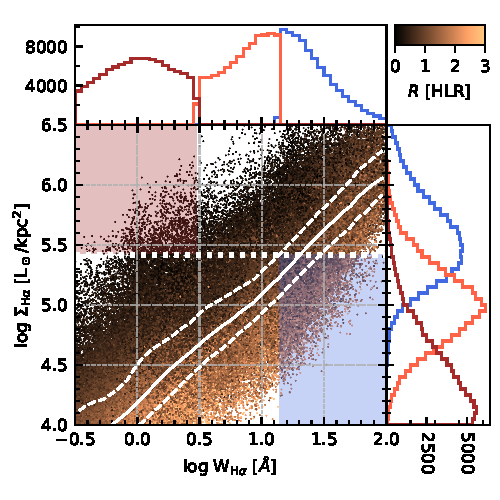
\includegraphics[scale=1.5]{figuras/fig_logSBHa_logWHa_histograms.pdf}
 \caption[$\log \Sigma_{{\rm H}\alpha} \times \log W_{{\rm H}\alpha}$]
 {$\log \Sigma_{\Ha}$ em função de $W_{\Ha}$ para as zonas de nossa amostra. Os intervalos em ambos eixos estão limitados àqueles valores que utilizamos para saturar os mapas na Figura \ref{fig:ExampleMaps}. Os pontos estão coloridos conforme a distânciada até o núcleo (em unidades de HLR). Os histogramas de $\Sigma_{\Ha}$ e de $W_{\Ha}$ estão coloridos com as mesmas cores utilizadas naqueles na Figura \ref{fig:WHa-Xi}. A linha contínua e as linhas tracejadas em branco marcam a mediana e o intervalo interquartil respectivamente. O limite $\Sigma^{\rm SF,min}_{\Ha} = 10^{39}$ erg$\,$s$^{-1}\,$kpc$^{-2}$ proposto por \citet{Zhang.etal.2017a} é sinalizando utilizando uma linha horizontal pontilhada branca. Um retângulo vermelho demarca a área onde há regiões classificadas como hDIG que possuem brilho superficial acima desse limite. Já a área onde caem aquelas regiões classificadas como SFc abaixo desse limite estão sobre um retângulo azul.}
 \label{fig:logWHa_logSBHa_histo}
\end{figure}
%---------------------------- Figure ----------------------------

Ao longo do disco da CALIFA 0886 a classificação utilizando o limite proposto por \citet{Zhang.etal.2017a} em $\Sigma_{\Ha}$ concorda com o regime nebular identificado por $W_{\Ha}$. Essa concordância ocorre apenas de forma parcial na CALIFA 0073 (painéis centrais na Figura \ref{fig:WHa_and_SHa_profiles}), onde encontramos mais regiões SF no disco utilizando o critério baseado em $W_{\Ha}$ do que aquele em $\Sigma_{\Ha}$. Esse fato é ainda mais acentuado na CALIFA 0813 (painéis inferiores), onde a maioria das regiões com $W_{\Ha} > 14$ \AA\ possuem $\Sigma_{\Ha}$ abaixo do limite $\Sigma^{\rm SF,min}_{\Ha}$. Essas diferenças se originam nos comportamentos radiais distintos entre $\Sigma_{\Ha}$ e $W_{\Ha}$.

Na Figura \ref{fig:logWHa_logSBHa_histo} podemos ver tudo isso de forma estatística. Os pontos representam as zonas em nossa amostra, coloridos por $R$. Vemos que para um valor de $W_{\Ha}$, as regiões mais brilhantes (maior $\Sigma_{\Ha}$) estão localizadas nas regiões centrais. Já para um valor fixo de $\Sigma_{\Ha}$, os maiores valores de $W_{\Ha}$ tendem a estar nos arredores. De fato, como vimos nos exemplos da Figura \ref{fig:WHa_and_SHa_profiles}, $\Sigma_{\Ha}$ tende a diminuir enquanto $W_{\Ha}$ se mantém mais ou menos constante, ambos com grandes dispersões em qualquer $R$ no disco. Cerca de 37\% das nossas regiões SFc possuem $\Sigma_{\Ha} < 10^{39}$ erg$\,$s$^{-1}\,$kpc$^{-2}$. Na média, essas regiões SFc pouco brilhantes estão localizadas em $R = 1.3$ HLR.

A área pintada em azul na Figura \ref{fig:logWHa_logSBHa_histo} marca regiões em que $\Sigma_{\Ha} < \Sigma^{\rm SF,min}_{\Ha}$, todavia com $W_{\Ha} > 14$ \AA, como vemos nos discos da CALIFA 0073 e na 0813. Se apoiando no exemplo da CALIFA 0886, vemos na área vermelha, regiões que seriam classificadas erroneamente utilizando o limite baseado em $\Sigma_{\Ha}$ proposto por \citet{Zhang.etal.2017a}.
\ED{\sout{Também podemos ver nessas áreas pintadas, agora com relevância estatística, esses casos onde regiões SFc com baixo brilho nas estão geralmente situadas nas regiões exteriores e regiões dominadas pelo regime hDIG, porém muito brilhantes, situadas em $R < 1$.}}
\ED{Também podemos ver, agora com relevância estatística, que regiões SFc com baixo brilho ocorrem nas partes exteriores das galáxias e que regiões dominadas pelo regime hDIG, porém muito brilhantes, estão situadas predominantemente nas zonas centrais ($R < 1$ HLR).}

Em resumo, comparado com o método de classificação em hDIG/mDIG/SFc baseado em $W_{\Ha}$ proposto neste trabalho, um critério baseado em $\Sigma_{\Ha}$ tende a sobrestimar a população de regiões SF situadas nas partes mais internas das galáxias. De maneira mais critica, como já foi mencionado, $\Sigma_{\Ha}$ não pode, por si só, identificar a componente hDIG, maior fonte de emissão em \Ha em  esferóides velhos.
\ED{\sout{Realmente temos visto que}}
\ED{Na verdade, vemos que}
bojos aposentados ({\em retired bulges}) muitas vezes são
\ED{\sout{classificados como}}
\ED{confundidos com} SFc quando seu brilho excede $\Sigma^{\rm SF,min}_{\Ha}$.

Trabalhos anteriores de utilizando dados do CALIFA por \citet{Kehrig.etal.2012}, \citet{Singh.etal.2013}, e \citet{Gomes.etal.2016b} também encontram valores $\Sigma_{\Ha}$, acima do limite $\Sigma^{\rm SF,min}_{\Ha}$ proposto por \citet{Zhang.etal.2017a}, nas regiões internas de galáxias {\em early-type}, onde incontestavelmente existe a ausência de estrelas jovens. (Veja também \citealt{Sarzi.etal.2010} para resultados baseados nos dados do SAURON\footnote{\em Spectrographic Area Unit for Research on Optical Nebulae survey}). Esses exemplos são realizações observacionais da inconsistência conceitual da soma de regiões DIG resultar em uma errônea classificação SF, apontada na Seção \ref{sec:DIGclass:WHaDistrib_hDIG}. O esquema apresentado nesta tese resolve esse problema extendendo para uma análise espacialmente resolvida, o conceito de galáxias aposentadas proposto por \citet{Stasinska.etal.2008a} e \citet{CidFernandes.etal.2011a} no contexto de espectros integrados.


\section{O DIG pode ser identificado por razões de linha sensíveis à densidade do meio?}
\label{sec:DIGdisc:nSii}

%---------------------------- Figure ----------------------------
\begin{figure}
 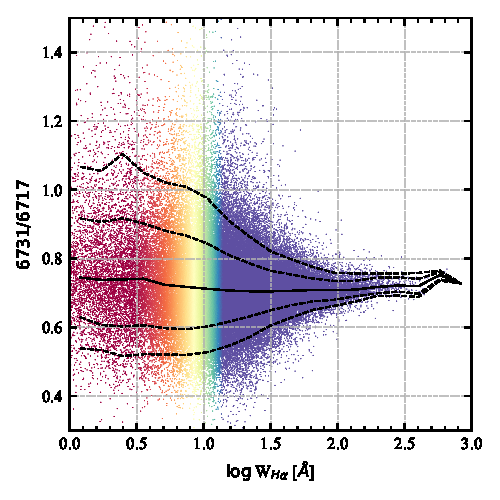
\includegraphics{figuras/fig_SII_logWHa_SNR3.pdf}
 \caption[$\log$ \sii$\times \log W_{{\rm H}\alpha}$]
 {Razão do fluxo de [S\,{\sc ii}]$\lambda\lambda$6731/6716 para $111\,760$ zonas em nossa amostra nas quais essa razão tem relação SN $\ge 3$. Pontos estão coloridos por $W_{\Ha}$ como nas figuras anteriores. A linha sólida representa a curva mediana, enquanto linhas tracejadas mostram o \ED{\sout{intervalos equivalentes a 1 e $2\sigma$}} \ED{5\textsuperscript{o}, 16\textsuperscript{o}, 84\textsuperscript{o} e o 95\textsuperscript{o} percentil} respectivamente.
 %{\ATR (percentis 5, 16, 84, e 95\%). [\ojo check!]}
 }
 \label{fig:S2_WHa}
\end{figure}
%---------------------------- Figure ----------------------------

As densidades eletrônicas do DIG na Via Láctea, obtidas através da combinação de medidas de dispersão e emissão e das colunas de densidade de \hi na direção de pulsares com distâncias conhecidas, são tipicamente abaixo de $10^{-1}$ cm$^{-3}$ \citep{Berk.and.Fletcher.2008}, ordens de magnitude menores que aqueles para regiões \hii.
As linhas do \Sii\ resultam da população através de excitação colisional de níveis muito próximos energeticamente e a razão da população dos níveis  é proporcional à densidade do meio.
Poderíamos então pensar que um estudo espacialmente resolvido da razão dessas linhas de \sii\ indicaria uma menor densidade nas regiões de DIG do que nos SFc. Nesse caso, tal razão mostraria uma tendência com $W_{\Ha}$.

Para testar isso inicialmente restringimos nossa amostra àquelas zonas onde SN $\ge 3$ na razão de linha \sii e mostramos na Figura \ref{fig:S2_WHa} a razão \sii 6731/6716 em função de $W_{\Ha}$. Nela vemos a curva mediana e os intervalos de 1 e 2$\sigma$ plotados. Não pudemos encontrar nenhuma relação entre a razão \sii 6731/6716 e $W_{\Ha}$. O aumento no espalhamento de pontos na direção de baixos $W_{\Ha}$ é consistente com a queda na relação SN das linhas. Mesmo nas regiões onde essa razão pode ser medida com segurança seu valor é $\sim 0.7$, limite inferior (baixa densidade) do intervalo sensível à densidade eletrônica através da razão \sii. Obviamente, essa figura não pode falar nada sobre as regiões onde SN < 3.

Nossa interpretação é que a razão de linhas \sii não nos mostra uma diferença quantitativa entre regiões DIG que puderam ter \sii medido e aquelas sob regime SFc por duas razões:
\begin{enumerate*}[label=(\roman*)]
    \item na resolução de nossos dados, as regiões SFc contém uma quantidade significativa de gás difuso;
    \item a razão de linhas \sii não é sensível à densidades menores que $\sim 50$\,cm$^{-3}$.
\end{enumerate*}

Poderíamos imaginar que um cenário diferente se formaria com estudos utilizando um dubleto sensível a baixas densidades, como o [N\,{\sc ii}]$\lambda\lambda$205,122\,$\mu$m, presente no infravermelho distante
%{\ATR (quais os lambdas?\ojo)}.
Observações recentes mapearam \ED{essas linhas}
%razão {\ATR [??QUE RAZAO??]}
na Via Láctea e outras galáxias \citep{Goldsmith.etal.2015, HerreraCamus.etal.2016}. As densidades derivadas \ED{pela razão entre elas} estão no intervalo de 1 a 300 cm$^{-3}$ com um valor mediano de 30 cm$^{-3}$. Esses valores não chegam perto das densidades do DIG obtidas por medidas através de pulsares.

Portanto concluímos que estimadores clássicos de densidade não são capazes de detectar o DIG, pelo menos não na resolução do CALIFA ou {\em surveys} simliares. Entretanto, não é bem certo se eles farão um melhor trabalho sob resolução espacial melhor pois, como percebido por \citet{Rubin.1989} sob outro contexto, inomogeneidades na densidade dificultam profundamente qualquer interpretação qualitativa de tais razões de linhas sensíveis à densidade do meio.


\section{$W_{{\rm H}\alpha}$ e o diagrama BPT}
\label{sec:DIGdisc:BPT}

%---------------------------- Figure ----------------------------
\begin{figure}
 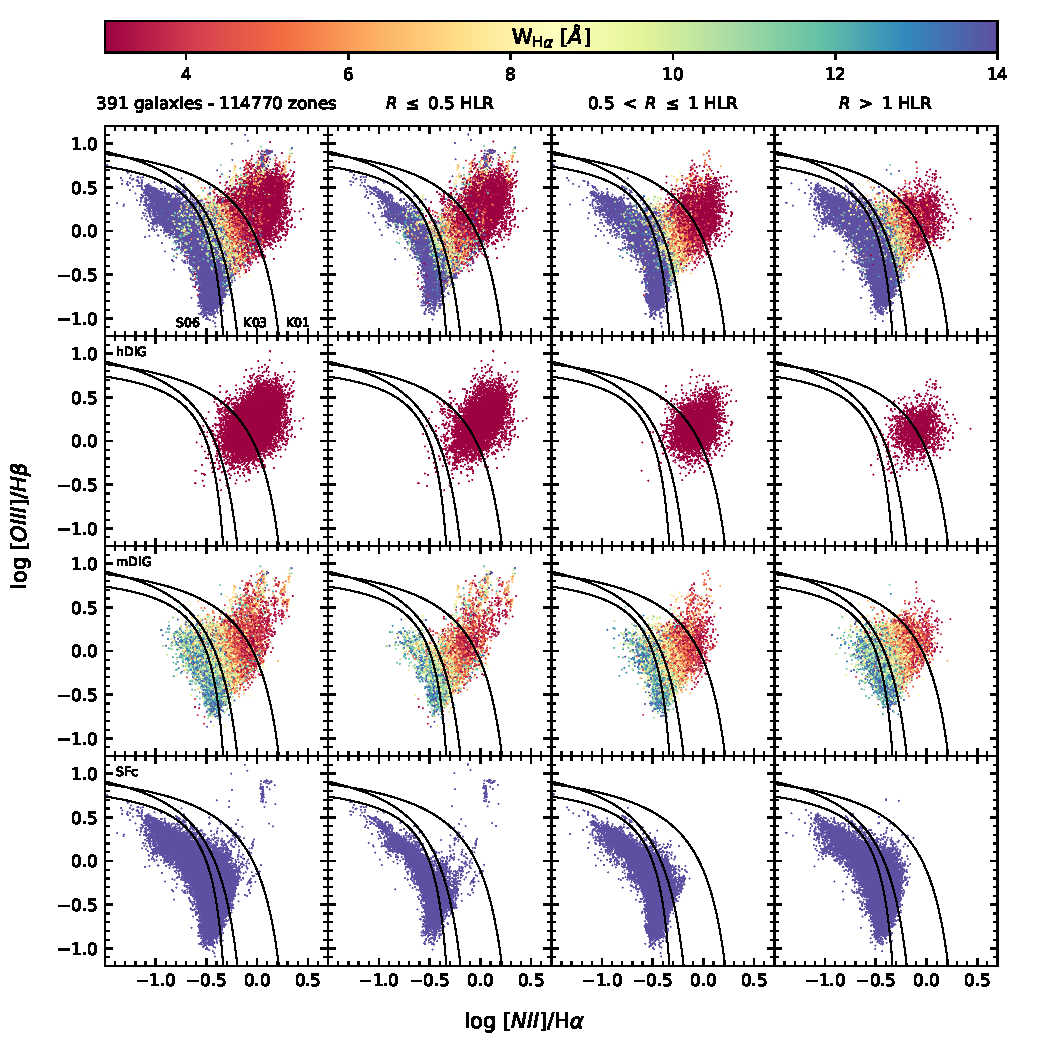
\includegraphics[scale=0.85]{figuras/fig_BPT_per_R.pdf}
 \caption[Diagramas BPT]
 {Diagrama BPT para nossa amostra. A primeira linha mostra todas as regiões em nossa amostra. Demais linhas dividem a amostra entre regiões SFc ($W_{\Ha} > 14$ \AA), mDIG ($W_{\Ha} = 3$--14 \AA), e hDIG ($W_{\Ha} < 3$ \AA). Em todos os painéis os pontos coloridos por $W_{\Ha}$ como indicado. Enquanto na primeira coluna temos os pontos para todas as posições das galáxias, nas seguintes os pontos são classificados de acordo com suas distâncias radiais, $R$, como na Figura \ref{fig:WHaDistrib_ALLgals}. Em todos os casos, plotamos apenas zonas com $SN \ge 3$ nas quatro linhas envolvidas. As curvas divisoras vêm de \citet[S06]{Stasinska.etal.2006a}, \citet[K03]{Kauffmann.etal.2003a}, e \citet[K01]{Kewley.etal.2001a} respectivamente.}
 \label{fig:BPT}
\end{figure}
%---------------------------- Figure ----------------------------

Diferentes processos de aquecimento e regimes de ionização no hDIG, mDIG e SFc devem resultar em diferentes razões entre fluxos de linhas colisionais e de recombinação, portanto distintas posições em diagramas de excitação como o  \Oiii/\Hb versus\ \Nii/\Ha. Esse famoso diagrama BPT \citep*[de][]{Baldwin.Phillips.Terlevich.1981a} é amplamente utilizado para separar galáxias SF daquelas onde uma fonte de ionização mais dura contribui de forma significante para a ionização do gás. Uma maneira de caracterizar regimes nebulares de forma independente serve de palco ideal para um teste de consistência da nossa classificação baseada em $W_{\Ha}$.

A Figura \ref{fig:BPT} mostra o diagrama BPT obtido para todas as zonas onde SN $\ge 3$ nas quatro linhas envolvidas. Os dados estão distribuídos de forma em que na coluna mais à esquerda estejam presentes regiões espalhadas em todas as partes das galáxias. Demais colunas separam regiões em três intervalos de distância radial como na Figura \ref{fig:WHaDistrib_ALLgals}. Na primeira linha vemos toda a amostra e, nas seguintes, os dados divididos entre hDIG/mDIG/SFc. Em todos os painéis os pontos são coloridos por $W_{\Ha}$ seguindo o mesmo esquema utilizado nos painéis da coluna da direita na Figura \ref{fig:ExampleMaps}. As curvas plotadas são aquelas propostas por \citet[S06]{Stasinska.etal.2006a}, \citet[K03]{Kauffmann.etal.2003a}, e \citet[K01]{Kewley.etal.2001a}. Essas curvas, teóricas ou empíricas, servem como divisórias demarcando distintos regimes de ionização no plano BPT---ver \citet{CidFernandes.etal.2011a} para uma discussão sobre o significado dessas curvas.

A forte correspondência entre $W_{\Ha}$ e as coordenadas no BPT é evidente, como foi previamente percebido por \citet{Morisset.etal.2016} com dados do CALIFA e \citet{Belfiore.etal.2016} com o MaNGA. A asa esquerda é predominantemente populada por regiões SFc, enquanto o hDIG se distribui pela asa direita, principalmente na ponta. Podemos notar que cada uma de nossas classes de regime de ionização preserva a área no plano BPT onde exerce uma predominância relativa, mesmo para diferentes intervalos de distância radial. Os pontos atípicos que aparecem nos dois painéis mais à esquerda na última linha, situados na região do plano BPT que é ocupado particularmente por regiões hDIG, se concentram nas regiões mais internas das galáxias. São regiões de nossa amostra onde $W_{\Ha}$ é alto mas são dominadas por ionização proveniente de um AGN, como será discutido na Seção \ref{sec:DIGdisc:caveats}.

Restringindo nossa análise para pontos onde $R > 1$ HLR (coluna mais à direita) para mitigar contaminação por regiões ionizadas por núcleos ativos, verificamos que 58\% (92\%) de nossas zonas com $W_{\Ha}$ > 14 \AA\ são classificadas como SF de acordo com o critério proposto por S06 (K03). O número relativamente grande de regiões SF que ultrapassam a linha de S06 não é surpreendente, já que a mesma foi traçada utilizando modelos de fotoionização desenvolvidos para estabelecer um limite para regiões puramente ionizadas por formação estelar. Como já argumentamos diversas vezes nesta tese, na resolução do CALIFA nossas regiões SFc não chegam nem perto de serem regiões \hii puras, por isso possuem bastante emissão difusa, o que acaba inflando ambas razões de linhas no diagrama BPT.

Concluímos portanto que nosso esquema de separação hDIG/mDIG/SFc leva a razões de linhas qualitativamente compatíveis com as quais deveríamos esperar em regiões sob tais regimes nebulares. Juntamente com os argumentos conceituais e empíricos apresentados na Seção \ref{sec:DIGclass:WHa}, essa análise utilizando o diagrama BPT reforça nossa metodologia.


\section{O mDIG como uma mistura de SF+hDIG}
\label{sec:DIGdisc:mDIG}

%---------------------------- Figure ----------------------------
\begin{figure}
 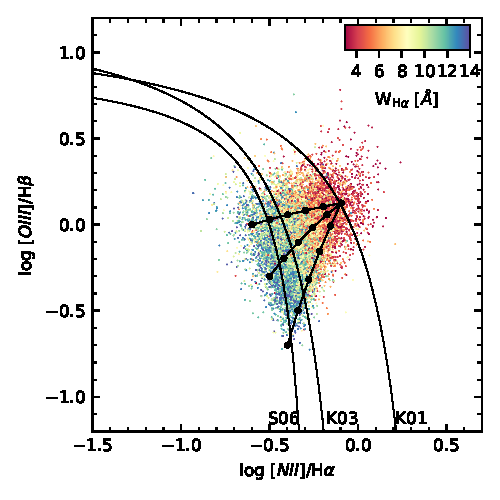
\includegraphics{figuras/fig_BPT_mixed_lines.pdf}
 \caption[Diagrama BPT -- mDIG]
 {Diagrama BPT filtrando apenas regiões mDIG (i.e., aquelas onde $W_{\Ha}$ está no intervalo 3--14 \AA), com pontos coloridos de acordo com $W_{\Ha}$, e excluindo zonas até $R = 1$ HLR.
 \ED{Linhas de mistura ligando as coordenadas medianas das regiões hDIG no plano BPT até três pontos ao longo da asa SF do BPT, com cículos pretos marcando os pontos onde a contribuição do hDIG para o fluxo de \Ha é igual a 0, 20, 40, 60, 80 e 100\%.}
 }
 \label{fig:BPT_mDIG}
\end{figure}
%---------------------------- Figure ----------------------------

Esta seção surge como um {\em addendum} à anterior, com a finalidade de explorar a natureza de emissão das regiões mDIG. A forma com que as regiões mDIG (penúltima linha da Figura \ref{fig:BPT}) se distribuem no diagrama BPT, entre a asa clássica das regiões SF e o local predominantemente populado por regiões hDIG, sugere uma interpretação em termos de uma mistura de fenômenos.
%Esse comportamento, por si só, já nos estimula a evocar tal cenário, porém podemos dizer mais utilizando o diagrama BPT.
A Figura \ref{fig:BPT_mDIG} trás em destaque o painel mais à direita da penúltima linha da Figura \ref{fig:BPT}. Nela vemos os pontos associados às regiões mDIG situadas em $R\ > 1$ HLR (= 5.3 kpc na média), coloridos por $W_{\Ha}$ como indicado.

A mesma progressão regular de $W_{\Ha}$ observada no painel do topo à esquerda na Figura \ref{fig:BPT} é observada na Figura \ref{fig:BPT_mDIG}, sugerindo fortemente um cenário composto pela mistura de emissão SFc e hDIG.
\ED{Nela adicionamos três linhas reforçando esta ideia. Estas são desenhadas ligando as coordenadas medianas dos pontos hDIG no BPT, $\log(\nii/\Ha,\oiii/\Hb) = (-0.09,+0.12)$, até três pontos ao longo da asa SF. Círculos pretos sobre essas linhas marcam pontos onde a contribuição hDIG para o fluxo de \Ha variam de 0 até 1, em passos de 0.2. Esse experimento indica que os locais no plano BPT ao longo da linha K03 (concebida para objetivos completamente diferentes) podem ser entendidos como uma mistura de emissão SFc e hDIG, onde SF contribui em $\sim 70\%$ para o fluxo total de \Ha, tendendo para 100\% hDIG sobre a linha K01. Naturalmente essas frações dependem do ponto pivô escolhido, todavia servem como um guia simples da mistura (veja também \citealt{Blanc.etal.2009} para um cenário análogo de mistura e seus efeitos nas estimativas da taxa de formação estelar).}

\ED{Que o mDIG é interpretável como uma mistura de processos é evidentemente o que alguém esperaria. O que talvez seja de alguma forma surpreendente é a relevância dos HOLMES nessa mistura. Intuitivamente esperaríamos que o gás difuso aquecido por fótons ionizantes que escapam de regiões \hii representaria um papel mais importante na constituição do mDIG. No entanto, há espaço para ambos cenários.} A população de regiões mDIG com $W_{\Ha}$ perto do limite de 14 \AA\ provavelmente corresponde a um cenário ionização devido ao escape de fótons de regiões SFc. De fato esses pontos se sobrepõem às coordenadas do BPT dominada por SFc. Acima da asa SF do BPT, o processo de ionização continua sendo principalmente governado por estrelas jovens e massivas, porém a influência do aquecimento por HOLMES aumenta gradativamente enquando $W_{\Ha}$ diminui. Quando $W_{\Ha}$ chega próximo ao limite de 3 \AA, o campo de radiação ionizante gerado por HOLMES começa a dominar o processo de fotoionização.

%{\ATR \ojo eu poria a fig com mixing lines ... ateh pra diferir um pouco + do paper!!}

%\section{AGN e outros {\em caveats}}
\section{AGN e outras fontes de linhas de emissão}
\label{sec:DIGdisc:caveats}

Nosso método de classificação hDIG/mDIG/SFc ignora outros mecanismos de produção de linhas. Dentre eles, o AGN é o mais notável. AGNs são encontrados nas partes centrais de galáxias e reconhecíveis através do diagrama BPT. Por exemplo, os pontos na ponta da asa direita com $W_{\Ha} > 14$ \AA\ na Figura \ref{fig:BPT} são provenientes das regiões internas da galáxias CALIFA 0897 (UGC 12348), ambas galáxias  Seyfert de tipo 2 \citep{Cusumano.etal.2010, Asmus.etal.2014}. Notamos que outros pontos erráticos que possuem $W_{\Ha} > 3$ \AA\ e situados em regiões internas ($R$ pequeno) tendem a ocupar a área do BPT geralmente ocupado por regiões hDIG.

AGNs podem prover energia para emissão de linhas em regiões muito distantes do núcleo (até distâncias de 20 kpc em casos extremos; \citealt{Veilleux.etal.2003}). Essas são conhecidas como EELRs ({\em extended emission-line regions}) ou cones de ionização. Esses cones podem ser originados por fotoionização de fótons de raio-X que deixam o núcleo com um pequeno ângulo de abertura ou por interação entre {\em radio jets} e o meio interestelar da galáxia produzindo fortes choques \citep{Wilson.1996}. Entretanto, na linha do presente estudo, a qual é avaliar a importância do DIG em galáxias em pontuar seus diferentes regimes, EELRs em galáxias Seyfert são um problema secundário, pois afetam apenas regiões específicas de galáxias com um AGN bem definido -- e talvez nem todas elas. Entender as EELRs é um tópico de estudo {\em per se} para ser investigado com espectroscopia 3D, e alguns estudos já começaram a fazê-lo \citep[e.g.,][]{Dopita.etal.2014}, porém está fora do escopo desta tese.

Choques estão também entre outros processos que podem gerar linhas de emissão e são negligenciados neste trabalho. No caso do vento galáctico na CALIFA 0811, presente na Figura \ref{fig:ExampleMapsEdgeOn}, encontramos $W_{\Ha}$ = 3--12 \AA\ na área de choque, i.e., valores presentes nas regiões que classificamos como mDIG. Novamente argumentamos que, por si só, $W_{\Ha}$  não pode identificar a origem dessa emissão nebular, apenas que fotoionização por HOLMES não é uma explicação factível. Somente um estudo detalhado da geometria, razões de linhas e cinemática desses objetos poderiam revelar os processos que governam a emissão de linhas nesses objetos \citep{Kreckel.etal.2014, Beirao.etal.2015, LopezCoba.etal.2017}. Devido ao seu número relativamente pequeno e por sua limitação espacial, tais objetos também não influenciam muito na estatística hDIG/mDIG/SFc presente neste estudo, entretanto não devem ser negligenciados em estudos de objetos individuais.

%{\ATR [\ojo falta algo nessa frase]
Finalmente, \ED{uma advertência/um aviso} sobre a tão conhecida região composta no BPT diagrama, comumente definida pela região abaixo da linha K01 e acima da K03 ou S06. Os objetos que ali se situam são interpretados geralmente como uma composição de SF + AGN. No entanto, AGN e hDIG possuem razões de linha indistinguíveis em diagramas de diagnóstico como o BPT. Portanto, a priori, não podemos afirmar realmente de que processos essa região é composta.

A forma de quebrar essa degenerescência é através de $W_{\Ha}$. Sabemos que estrelas velhas e quentes, diferentemente de AGN ou SF, ocupam toda a extensão de galáxias. Consequentemente, o regime hDIG deve ser considerado
%A radiação proveniente dos HOLMES, que produz $W_{\Ha} \sim 1$ \AA, deve portanto ser considerada
nível mínimo de ionização, ou seja, aquele que é energeticamente relevante quando nenhum outro é. Sempre que o contínuo ao redor de \Ha\ for dominado por estrelas velhas, que é o caso mesmo para regiões SF na resolução na casa de kpc, a razão entre o fluxo ionizante e aquele proveniente do contínuo estelar deve gerar valores de $W_{\Ha} \sim$ 1--2 \AA\ de acordo com os modelos de população estelar (ver \citealt{CidFernandes.etal.2011a}). Logo, espectros que possuam $W_{\Ha}$ próximo desse valor e caiam na região composta do BPT certamente representam uma mistura SFc + hDIG. Entretando, enquanto $W_{\Ha}$ estiver acima do intervalo hDIG, uma mistura formada por SF + AGN é mais plausível.

O estudo de \citet{Davies.etal.2014} ilustra este ponto. Usando cubos de dados do CALIFA de quatro galáxias, duas  Seyfert (NGC 2410 e NGC 6394) e outras duas onde a classificação Seyfert--LINER é incerta (IC 0540 e NGC 6762), eles identificam distribuições praticamente unidimensionais no diagrama BPT e outros diagramas de excitação. Essas distribuições sugerem uma sequência de mistura SF + AGN. No entanto eles verificaram que em NGC 6762 a maioria (> 90\%) dos {\em spaxels} possuem $W_{\Ha} < 3$ \AA\ e, por essa razão, a contribuição de HOLMES não pode ser ignorada. Por outro lado, as galáxias NGC 2410 e NGC 6394 possuem regiões centrais com $W_{\Ha}$ bem acima do limite de hDIG, portanto uma mistura SF + AGN é mais provavel. Na IC 0540 os valores de $W_{\Ha}$ estão no intervalo hDIG--mDIG, o qual torna qualquer interpretação sob estes argumentos menos exata,
\ED{embora eles favoreçam um cenário de mistura SF + AGN.}
%{\ATR embora eles pendam para uma mais favorável à mistura SF + AGN. [\ojo reword]}
Cremos que o ponto principal aqui é que $W_{\Ha}$ deve ser levado sempre em conta em estudos de sistemas compostos a fim de evitarmos confusão entre os efeitos do hDIG e de AGN.

%%%%%%%%%%%%%%%%%%%%%%%%%%%%%%%%%%%%%%%%%%%%%%%%%%%%%%%%%%%%%%%%%
% Tese de Doutorado / Dept. Fisica, CFM, UFSC                   %
%%%%%%%%%%%%%%%%%%%%%%%%%%%%%%%%%%%%%%%%%%%%%%%%%%%%%%%%%%%%%%%%%

%:::::::::::::::::::::::::::::::::::::::::::::::::::::::::::::::%
%                                                               %
%                          Capítulo 5                           %
%                                                               %
%:::::::::::::::::::::::::::::::::::::::::::::::::::::::::::::::%

%***************************************************************%
%                                                               %
%                          Conclusão                            %
%                                                               %
%***************************************************************%

\chapter{Conclusões e perspectivas}
\label{sec:concl}

\ED{Vamos revisar os principais resultados dos Capítulos 2--4 neste capítulo, além de apresentar alguns dos projetos que figurarão entre nossos próximos estudos, tanto no CALIFA quanto no MaNGA. Muitos dos problemas não resolvidos pela astrofísica ainda dependem de avanços tecnológicos em todas as áreas, desde observação até processamento e armazenamento de dados. Junto às perspectivas aqui apresentados dos próximos estudos sobre o DIG, mostro um exemplo de artigo com um estudo isolado utilizando dados do MUSE. Trabalhos como esse irão revolucionar mais uma vez as descobertas de nossa área.}

%{\ATR \ojo Falta aqui um preambulozinho como tem em todos outros capitulos.  Algo do tipo : vamos revisar os princiapis resultados dos caps 2--4, e apresentar outras cousas que trabalhamos e estamos trabalhando.}

\section{DIG no CALIFA: a classificação}
\label{sec:concl:DIGCALIFA}
No artigo principal desta tese utlizamos uma amostra de $307\,958$ zonas de 391 galáxias do CALIFA Survey dos mais variados tipos de Hubble. Estudos baseados em espectros integrados, como os do \SDSS, tiveram grande importância na determinação da existência ou não de núcleos ativos em galáxias. Em uma amostra espacialmente resolvida como a nossa, um questionamento mais relevante seria veririficar o regime de ionização de cada região é dominado por fótons que escapam de estrelas massivas (seja por regiões \hii ou pelo gás difuso que as circulam) ou por fótons criados por populações estelares velhas. E esta é a linha principal do artigo \citet[][Apêndice \ref{apendice:DIGpaper0}]{Lacerda.etal.2018} e desta tese.
% \ojo
% %\citet[]{Apêndice \ref{apendice:DIGpaper0}}
% \ref{apendice:DIGpaper0} e desta tese.

Nesse trabalho mostramos que o método comumente adotado de seleção de regiões SF/DIG baseado no brilho sperficial de \Ha, $\Sigma_{\Ha}$, é conceitualmente falho. Mostramos que  através da largura equivalente de \Ha, $W_{\Ha}$, esses dois regimes são diferenciados qualitativamente de uma maneira mais evidente. Além disso, talvez de forma mais importante, $W_{\Ha}$ consegue identificar os casos onde o regime de ionização é dominado por HOLMES, uma população estelar omnipresente que serve de nível mínimo de radiação ionizante em galáxias.

Propusemos uma classificação baseada na distribuição observada de $W_{\Ha}$ entre e ao longo das galáxias. As regiões onde $W_{\Ha} \le 3$ \AA\ foram classificadas como ionizadas por HOLMEs (hDIG), que são responsáveis pelo pico de 1 \AA\ na distribuição fortemente bimodal de $W_{\Ha}$. Essa definição observacional do hDIG é idêntica àquela para galáxias aposentadas \citep{CidFernandes.etal.2011a}.
Na falta de um argumento (astro)físico, criamos o conceito de complexos de formação estelar, SFc, definido como regiões onde $W_{\Ha} > 14$ \AA, a moda da população com alto $W_{\Ha}$ em nossa amostra. As regiões com valores intermediários chamamos de DIG misto (mDIG).

%A seguir alguns dos principais resultados obtidos com este estudo {\ATR motivado tanto teoricamente quanto empiricamente. [\ojo hmmm... soa meio feio...]}
A seguir alguns dos principais resultados obtidos com este estudo motivado tanto
\ED{\sout{teoricamente}} \ED{teórica} quanto empiricamente.

\begin{enumerate}[label=(\roman*)]
  \item Em acordo com suas populações estelares, que são predominantemente velhas, o hDIG é o regime de ionização prevalente em galáxias {\em early-type}.
  \item A emissão extraplanar em galáxias espirais {\em edge-on} também é hDIG, sustentando o cenário proposto e elaborado por \citet{FloresFajardo.etal.2011a}.
  %Em sistemas {\em face-on} a emissão extraplanar hDIG é parte {\ATR negligenciável relativamente quando estamos sob regime SFc [\ojo reword]}.
  Em sistemas {\em face-on} a emissão extraplanar hDIG é
  \ED{\sout{parte negligenciável relativamente quando estamos sob regime SFc.}}
  \ED{relativamente negligenciável quando estamos observando regiões SFc.}
  Já quando é projetada sobre regiões classificadas como mDIG essa contribuição é potencialmente relevante.
  \item Uma classificação SF/DIG baseada em $\Sigma_{\Ha}$ tende a classificar bojos aposentados dominados por hDIG como SFc, uma incosistência criada por construção pela natureza extensiva de $\Sigma_{\Ha}$.
  \item A contribuição percentual para a luminosidade de \Ha proveniente dos regimes hDIG, mDIG e SFc varia entre (100, 0, 0)\% para sistemas elípticos e S0, passando por (9, 60, 31)\% em galáxias Sa--Sb até (0, 13, 87)\% para tipos mais tardios.
  \item As regiões SFc e hDIG ocupam locais bem definidos no diagrama BPT independentemente da distância radial ao núcleo da galáxia, $R$. As regiões mDIG, se espalham por todo o plano BPT, porém se concentrando mais na parte conhecida como composta (entre as linhas K01 e K03), formando uma sequência contínua entre as razões de linha SFc e hDIG, indicativo de um cenário de mistura mDIG = SFc + hDIG.
\end{enumerate}

\section{Outros trabalhos}
\label{sec:concl:other}

Antes do estudo sobre as regiões DIG no CALIFA participei de outros estudos espacialmente resolvidos envolvendo populações estelares e linhas de emissão. Como primeira etapa construí uma classe em \pyt, descrita no Apêndice \ref{apendice:EmLinesDataCube}, que permitiu os estudos descritos no Apêndice \ref{apendice:synvsneb} onde comparamos propriedades estelares e nebulares. Esses estudos fizeram parte da discussão de diversos artigos no CALIFA. Parte dessa pesquisa, em particular das comparações entre da taxa de formação estelar proveniente da síntese e aquela estimada pela luminosidade de \Ha, foi publicada no artigo \citep{GonzalezDelgado.etal.2016a}, e também utilizado em comparações nos artigos \citet{CortijoFerrero.etal.2017a, CortijoFerrero.etal.2017b, CortijoFerrero.etal.2017c}.

Também participei dos estudos de controle de qualidade para o segundo lançamento público de dados do CALIFA  \citet[DR2; ][Apêndice \ref{apendice:GBetal2015a}]{GarciaBenito.etal.2015a}. Repetimos essa análise para o DR3 e comparações com os resultados das amostras anteriores mostraram uma gradativa melhora nos erros estimados pela pipeline de redução do CALIFA, resultando em melhores espectros residuais e máscaras de linhas de emissão utilizadas na síntese.


\section{Perspectivas futuras -- O futuro próximo do IFS}
\label{sec:concl:futIFS}

\subsection{DIG no MaNGA: a fração relativa do fluxo de linhas de emissão referente ao DIG -- $f_\lambda^{\rm DIG}$}
\label{sec:concl:futIFS:DIGMaNGA}
Estudos que utilizam espectros integrados (i.e., não resolvidos espacialmente) como aqueles do \SDSS negligenciam a contribuição fracional de cada regime de ionização para o fluxo das linhas de emissão. Quando a intenção é calcular a taxa de formação estelar através da luminosidade de \Ha (ver Seção \ref{apendice:EmLinesDataCube:props:SFR}) temos que considerar apenas os fótons ionizantes provenientes de estrelas massivas. Similarmente, ao estimar a abundância relativa de oxigênio de galáxias SF, fica impossível descontar a contribuição do DIG para o fluxo das linhas de emissão necessárias para o cálculo de O/H (veja \citealt{Sanders.etal.2017a} e referências ali) utilizando dados integrados.

%---------------------------- Figure ----------------------------
\begin{figure}
	\centering
	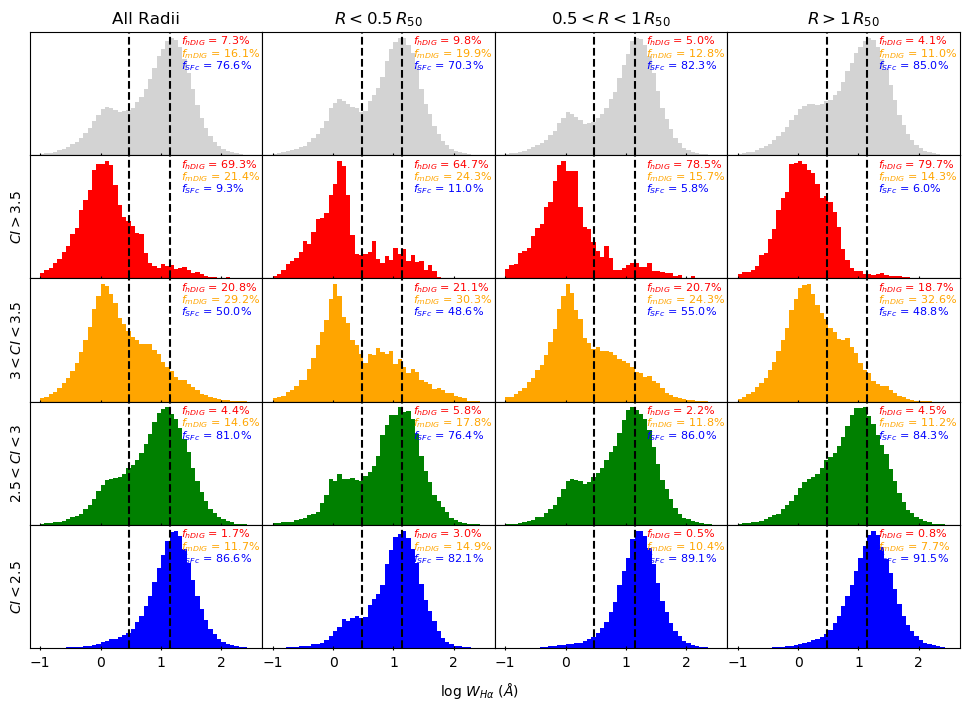
\includegraphics[scale=0.5]{figuras/fig_WHa_histo_per_CI_and_R_cumulFHa_MaNGA.png}
	\caption[MaNGA: Histogramas de $W_{{\rm H}\alpha}$]
	{Como a Figura \ref{fig:WHaDistrib_ALLgals} entretanto para a amostra do MaNGA. Nesta figura, o índice de concentração, CI, {\ATR definido como...\ojo]} é utilizado como um indicador de morfologia das galáxias.
{\ATR Figura preparada por G. Couto...}
	}
	\label{fig:WHaDistrib_ALLgals_MaNGA}
\end{figure}
%---------------------------- Figure ----------------------------

Com uma amostra estatisticamente mais robusta, utilizando dados espacialmente resolvidos do MaNGA, nossa intenção é aplicar o mesmo método de classificação de \citet[][Apêndice \ref{apendice:DIGpaper0}]{Lacerda.etal.2018} de forma a analisar a contribuição relativa do DIG para os  fluxos de diferentes linhas de emissão, $f_\lambda^{\rm DIG}$, e calibrar essas frações em função de propriedades integradas de galáxias de maneira que possamos usá-las para corrigir os espectros pela emissão DIG. A Figura \ref{fig:WHaDistrib_ALLgals_MaNGA} mostra que a bimodalidade em $W_{\Ha}$ se mantém para essa amostra maior e que a prevalência de cada classe para cada tipo morfológico (aqui representada pelo índice de concentração CI) também é semelhante. Isso mostra que a metodologia desenvolvida nessa tese pode também ser aplicada a dados MaNGA.

%---------------------------- Figure ----------------------------
\begin{figure}
	\centering
	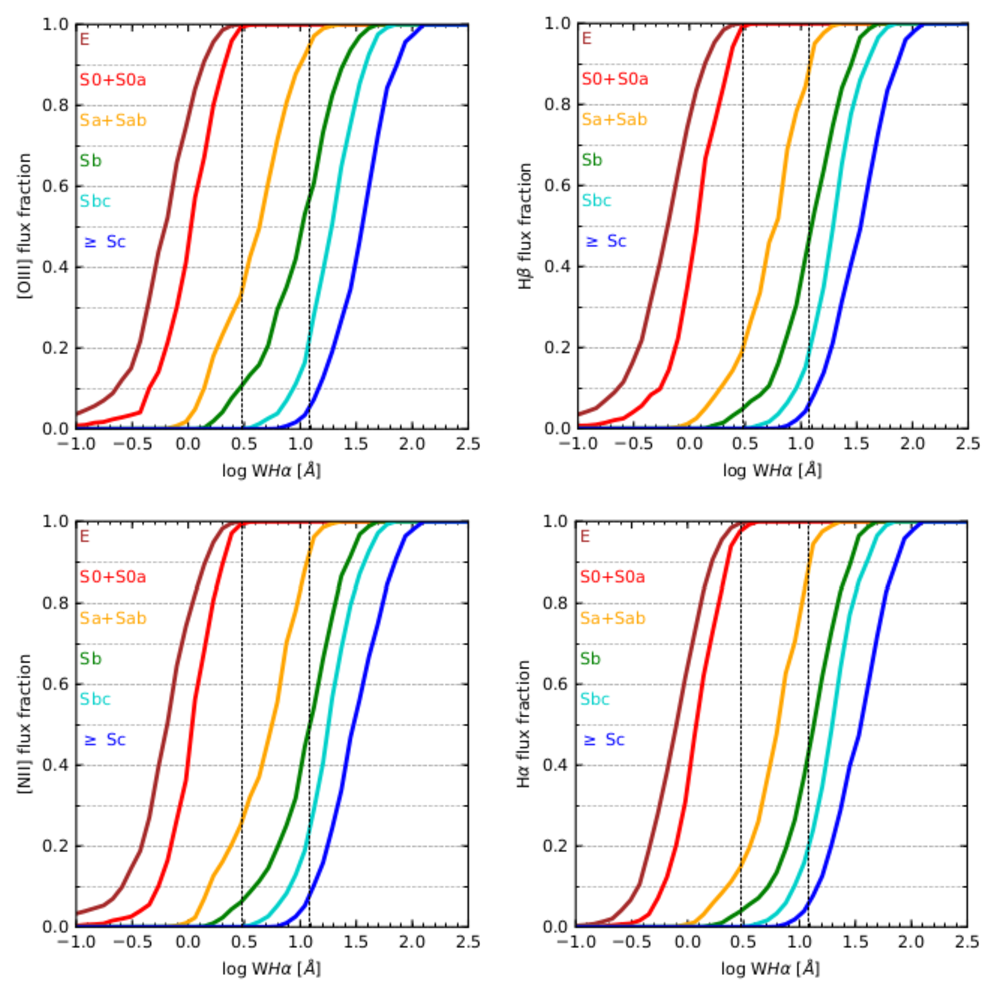
\includegraphics{figuras/bptlines_fracDIG.pdf}
	\caption[Contribuição de DIG para os fluxos das linhas do BPT]
	{Como a Figura \ref{fig:CurveOfGrowth} porém para o fluxo total das linhas utilizadas no diagrama BPT.}
	\label{fig:bptlines_fracDIG}
\end{figure}
%---------------------------- Figure ----------------------------

Os experimentos com frações de DIG para diferentes linhas de emissão já foi feito para o CALIFA durante esta primeira etapa do trabalho, como podemos ver na Figura \ref{fig:bptlines_fracDIG}. Essa figura é como a figura \ref{fig:CurveOfGrowth}, onde avaliamos como a fração do fluxo para determinada linha se altera com o crescimento de $W_{\Ha}$.
{\ATR \ojo mais uma ou duas frases pra fechar!}


\subsection{Estatística com melhor resolução espacial}
\label{sec:concl:futIFS:MUSE}
\begin{figure}
 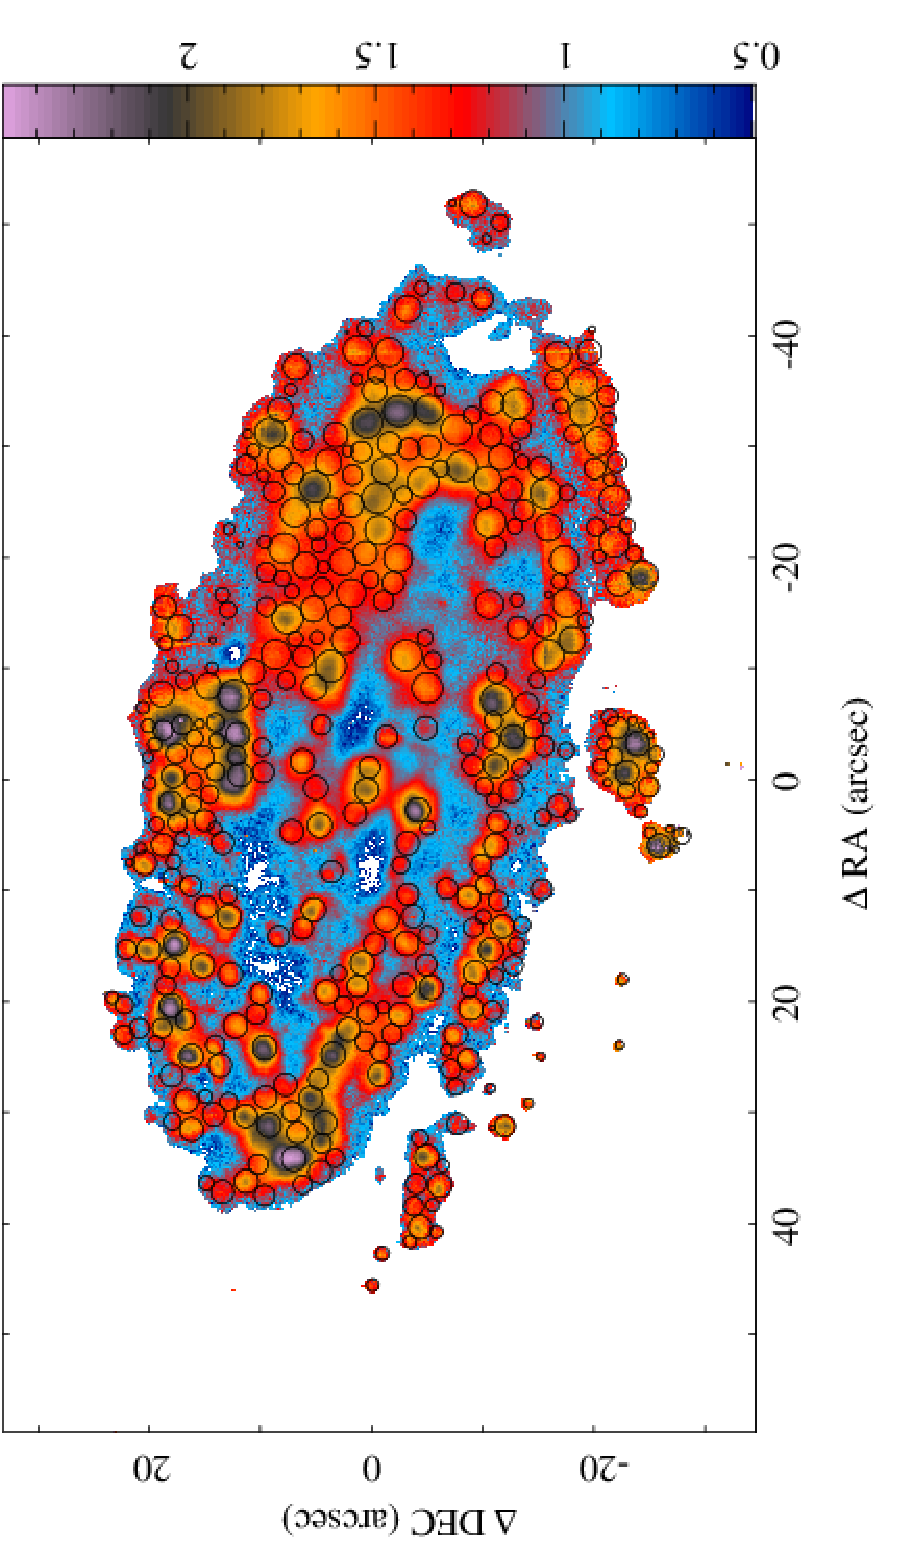
\includegraphics[scale=0.5,angle=-90]{figuras/map_EW_Ha_HII.pdf}
 \caption[MUSE: Mapa de $W_{{\rm H}\alpha}$ da galáxia NGC 6754]
 {Mapa da galáxias NGC 6754 obtido por \citet{Sanchez.etal.2015MUSE} colorido por $\log\ W_{\Ha}$. Regiões com detecção de fluxo de \Ha abaixo de $\sim 3\sigma$ são mascaradas. Os circulos marcam regiões \hii detectadas.}
 \label{fig:WHaSebasMUSE}
\end{figure}

Referencio aqui o trabalho de \citet{Sanchez.etal.2015MUSE}, um exemplo de estudo embasado em imagens com uma resolução espacial muito maior, obtidas com o MUSE. São $\sim 200\,000$ espectros amostrando cada parte da galáxia até dois raios efetivos, cobrindo uma área de $\sim 2' \times 1'$ arcmin$^2$. A resolução espacial é muito melhor que a maioria dos {\em surveys} atuais de IFS, e com uma análise individual de cada espectro podemos construir mapas como o de $W_{\Ha}$ da galáxia NGC 6754, reproduzido aqui na Figura \ref{fig:WHaSebasMUSE}. Essa figura mostra um domínio completo de regiões SFc permeadas por emissão mDIG em todo disco.
{\ATR \ojo falta um ??e daí??}

% \subsection{Mascarando elementos e removendo {\em outliers}}
% \label{sec:sample:mask}
%
% Para que possamos focar nossos estudos nas regiões de formação estelar, aplicamos uma máscara nos
% dados selecionando as regiões que possuam:
% \begin{itemize}
%   \setlength\itemsep{0.2cm}
%   \item medidas do fluxo integrado das linhas de \Hbeta, \oIII, \Halpha e \nII com relação
% sinal-ruído maior do que 3;
%   \item medidas para as seis propriedades comparadas neste capítulo:
%   \begin{itemize}
%     \item coeficiente de extinção proveniente da síntese - $\tauVS$;
%     \item coeficiente de extinção estimado através do decremento de Balmer - $\tauVN$;
%     \item densidade superficial da taxa de formação estelar calculado através da síntese -
% $\SigmaSFR$;
% 	\item densidade superficial da taxa de formação estelar calculado através da luminosidade de
% \Halpha - $\SigmaSFRN$;
% 	\item metalicidade média das populações estelares, pesada pela massa estelar - $\meanM{\log
% Z_\star}$;
% 	\item metalicidade nebular - $\log(O/H)$.
%   \end{itemize}
%   \item fração de luz proveniente de populações estelares jovens maior que 0.05 (5\%) ($x_Y >
% 0.05$);
%   \item $\tauV$ e $\tauVN$ maiores que 0.05;
%   \item mais do que cinco zonas contribuindo para o cálculo dos perfis radiais;
%   \item distância ao núcleo maior que 70\% do raio que contém metade da luz ({\em half-light
%  radius} - HLR) e menor que 3 HLR.
% \end{itemize}
% \noindent O que aqui chamamos de população jovem discutiremos um pouco mais adiante, na Sec.
% \ref{sec:synvsneb:SFR}. A última imposição é feita para que não haja contaminação por zonas
% do bojo da galáxia (partes centrais onde as linhas são produzidas por diferentes fenômenos físicos,
% relacionados a um núcleo ativo). Esse valor (0.7 HLR) foi definido por nossos colaboradores
% analisando as curvas de brilho das galáxias e representa um valor máximo para localização de zonas
% centrais.
%
% Na Fig.\ \ref{fig:histosample} podemos ver os histogramas normalizados (a integral dentro do
% intervalo do histograma é 1) de algumas propriedades de modo que evidencie os efeitos da máscara
% que forma nossa amostra. Em vermelho temos as 226176 regiões em 305 galáxias e, em azul, as 16479
% zonas de 184 galáxias (19 Sa, 38 Sb, 59 Sbc, 55 Sc e 13 Sd). É notável que nossa seleção busca zonas
% mais densas e mais jovens (maior fração de populações jovens diminuindo a idade média). O corte mais
% brusco em nossa amostra é devido a baixa relação sinal-ruído da linha de \oIII ($S/N_{\oIII} < 3$)
% em 91142 zonas.
% \begin{figure}
% 	\centering
% 	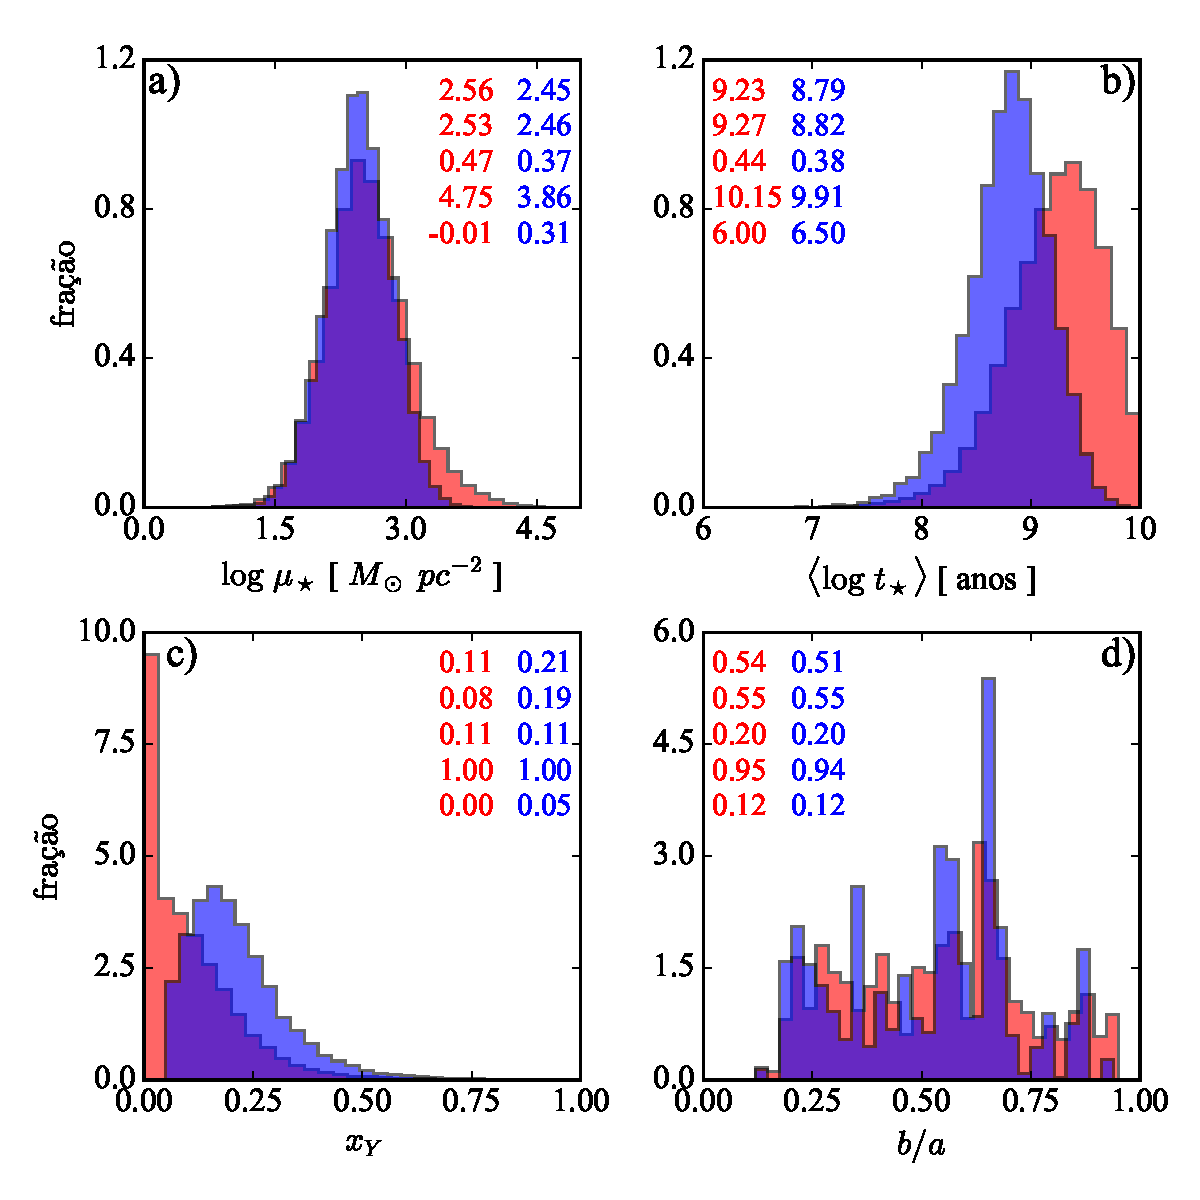
\includegraphics[width=0.99\textwidth]{figuras/histosample.pdf}
% 	\caption[Histogramas: densidade superficial de massa, idade média, fração de populações jovens e
% 	relação axial.]
% 	{Histogramas da densidade superficial de massa ({\em painel a}), idade média das populações
% estelares ({\em painel b}), fração em luz proveniente de populações jovens ($x_Y \equiv x_Y(t_\star <
% 31.62$ milhões de anos, {\em painel c}) e relação axial ({\em painel d}). Em vermelho temos a
% distribuição de valores de 226176 regiões em 305 galáxias e, em azul, a de 16479 zonas de 184
% galáxias resultantes da seleção. Em cada gráfico temos os valores da média, mediana, desvio padrão,
% máximo e mínimo de cada distribuição.}
% 	\label{fig:histosample}
% \end{figure}
%
% \subsection{Classificação Morfológica}
% \label{sec:sample:morf}
%
% Com tipos morfológicos variando entre Sa e Sd, massas estelares entre $10^9$ e $10^{11.5}\ M_\odot$
% e populações estelares com idades médias entre $10^8$ e $10^{10}$ anos, podemos ver na Fig.
% \ref{fig:amostraMorf} que as galáxias se ordenam de forma interessante quando agrupadas por tipo
% morfológico, anticorrelacionando com a idade média estelar e a massa estelar ($M_\star$ e $t_\star$)
% e correlacionando com a fração de luz proveniente das população jovens ($x_Y \equiv x_Y(t_\star <
% 31.62$ milhões de anos)). Cada galáxia contribui com um ponto em cada painel deste gráfico, ou seja,
% são propriedades integradas. Os intervalos entre primeiro e terceiro quartil quase não se sobrepõem
% quando analisamos as classes morfológicas por idade média.
%
% Esse resultado parece ser interessante visto que a classificação morfológica foi feita por
% colaboradores do CALIFA totalmente através de inspeção visual das imagens na banda-r do \SDSS das
% mesmas galáxias. Vemos também que as galáxias tipo Sd possuem as populações estelares mais jovens e
% menos massivas na média. Por ser um fenômeno apenas de posição do referencial de observação não
% deveríamos ver preferência por valor de relação axial ($b/a$) quando dividimos em classes
% morfológicas, o que realmente acontece.
%
% \begin{figure}
% 	\centering
% 	\includegraphics[width=0.99\textwidth]{figuras/sample_realsample_maskradius_integrated.pdf}
% 	\caption[Classificação por morfologia]
% 	{Valores integrados das mesmas propriedades da Fig.\ \ref{fig:histosample} para as 184
% galáxias da amostra, separadas em classes morfológicas. No primeiro painel, temos o número de
% galáxias dentro de cada classe morfológica. Cada caixa tem altura definida pelo primeiro e terceiro
% quartil da distribuição dentro de um tipo morfológico. Uma faixa preta marca a mediana e uma
% estrela a média. Em cada caixa, a linha pontilhada vertical se estende mostrando o intervalo de
% $3\sigma$. Valores que ficam fora do intervalo de $3\sigma$ são marcados por uma cruz vermelha.}
% 	\label{fig:amostraMorf}
% \end{figure}
%
% Estamos em fase de finalização de um artigo em que comparamos a relação entre a taxa de formação
% estelar e a massa para diferentes classes morfológicas. Esse artigo já foi submetido e deve sair
% logo agora no início de 2016.
%
%
%
%
%
%
% \section{Perfis radiais}
% \label{sec:amostra:rad}
%
% Uma maneira interessante de analisar galáxias é produzir perfis radiais para as propriedades
% físicas. Esse tipo de média azimutal (tanto em classes definidas por anéis circulares quanto em
% anéis elípticos) diminui o espalhamento dos pontos. Para a análise individual de cada galáxia também
% permite estudo da evolução das propriedades ao longo do raio. Quando colocamos todas as galáxias na
% mesma análise, a vantagem dos {\em bins} radiais vem do balanceamento da influência de cada galáxia
% quando analisamos todas juntas. Para que seja possível este ``empilhamento'' de galáxias, estas
% médias radiais são feitas definindo-se um raio efetivo para cada galáxia. No nosso caso utilizamos
% como raio efetivo aquele que comporta metade da luz da galáxia (HLR) e definimos 30 anéis com
% espessura de 0.1 HLR (ou seja, indo até 3 HLR) partindo do pixel central de cada galáxia.
%
% No artigo de \citet{GonzalezDelgado.etal.2014a} os autores discutem as estruturas radiais de algumas
% propriedades estelares, aplicando este tipo de estudo para 107 galáxias no CALIFA. Nele são
% derivados os raios que contém metade da luz (HLR) e metade da massa ({\em half-mass radius} - HMR) e
% deste resultado concluem que as galáxias são em geral 15\% mais compactas em massa do que em luz.
% Também mostram que algumas propriedades, como idade estelar média, extinção por poeira e densidade
% superficial de massa estelar são bem representados pelo seus valores medidas a 1 HLR.
%
% Escolhemos utilizar perfis radiais em anéis elípticos neste trabalho, calculando a média entre todas
% as zonas não mascaradas dentro de cana anel em cada galáxia. Como um exemplo, podemos observar na
% Fig.\ \ref{fig:K0140xYRadProf} três exemplos de mapas e perfis radiais ($x_Y$, $\tauVS$ e $\tauVN$)
% da galáxia NGC1667 (objeto CALIFA 140). Em destaque (azul) temos o valor integrado para a galáxia.
% Dentro de nosso trabalho utilizamos as medidas em zonas, em perfis radiais e quando necessário,
% integradas (resolvendo para o disco ou para a galáxia completa), nos possibilitando portanto
% verificar diferenças nestes tipos de abordagens.
%
% \begin{figure}
% 	\centering
% 	\includegraphics[width=0.99\textwidth]{figuras/K0140_xY_radialProfile_realsample.pdf}
% 	\caption[Imagem e exemplos de mapas e perfis radiais]
% 	{Imagem do \SDSS da galáxia NGC1667 (CALIFA 140). Em cada fileira aparece o mapa e o perfil radial
% da fração de luz proveniente das populações jovens ($x_Y$ - \emph{primeira fileira}), do
% coeficiente de extinção resultante da síntese de populações estelares ($\tauVS$ - \emph{segunda
% fileira}) e do coeficiente de extinção por decremento de Balmer ($\tauVN$ - \emph{terceira
% fileira}). Nos mapas duas elipses concêntricas marcam 1 e 2 HLR. Em cada gráfico do perfil radial
% aparece no fundo em cinza os valores para as zonas, em linha tracejada preta a mediana da
% distribuição ao longo do raio e em azul tracejado o valor integrado para a galáxia, além do perfil
% radial (linha preta contínua).}
% 	\label{fig:K0140xYRadProf}
% \end{figure}
%
% O perfil radial médio das principais propriedades utilizadas neste trabalho podem ser vistas na
% Fig.\ \ref{fig:RadProfProps} juntamente com seus histogramas na Fig. \ref{fig:HistoRadProfProps}.
% Note que estamos apenas colocando os pontoa onde o reaio esteja entre 0.7 e 3 HLR. Elas são muito
% importantes em todos os aspectos que abordaremos: formação estelar, poeira e a conversão de
% densidade superficial de poeira em densidade superficial de gás em discos de galáxias espirais.
% Podemos ver que existem alguns gradientes negativos (crescem de fora para dentro) bem definidos de
% densidade superficial da taxa de formação estelar ($\Sigma_{\mathrm{SFR}}$), a metalicidade nebular,
% ($\log O/H$), densidade superficial de massa estelar ($\mu_\star$). Outras propriedades parecem não
% variar muito dentro do disco. Alguns perfis mudam de tendência ao passar de 2 HLR, mas vale
% ressaltar que na maioria das distribuições, os pontos acima de 2 HLR ultrapassam $1\sigma$ da
% distribuição. Embora não seja tão forte, existe um gradiente positivo na fração em luz de populações
% jovens.
%
% \begin{figure}
% 	\centering
% 	\includegraphics[width=0.9\textwidth]{figuras/props_R.pdf}
% 	\caption[Perfis radiais das propriedades físicas]
% 	{Perfis radiais médios (entre 0.7 e 3 HLR) das principais propriedades físicas abordadas neste
% trabalho. Densidade superficial da taxa de formação estelar detectada por \Halpha e pela síntese
% ({\em painéis a e b}), idade média das populações estelares ({\em painel c}), metalicidade nebular
% ({\em painel d}), fração em luz de populações jovens ({\em painel e}), densidade superficial de
% massa estelar ({\em painel f}), metalicidade média das populações estelares ({\em painel g}),
% coeficiente de extinção da síntese e do decremento de Balmer ({\em painéis h e i}). Em cada painel
% vemos também os contornos definindo $1\sigma$, $2\sigma$ e $3\sigma$ da distribuição. As linhas
% marcam a mediana (linha contínua) e os 5, 16, 64, 95 percentis (linhas tracejadas).}
% 	\label{fig:RadProfProps}
% \end{figure}
%
% \begin{figure}
% 	\centering
% 	\includegraphics[width=0.99\textwidth]{figuras/histo_props_R.pdf}
% 	\caption[Histogramas dos perfis radiais das propriedades físicas]
% 	{Histogramas normalizados de todas as propriedades físicas da Fig.\ \ref{fig:RadProfProps}. Os
% valores no canto superior direito marcam a média, mediana, desvio padrão, máximo e mínimo das
% distribuições.}
% 	\label{fig:HistoRadProfProps}
% \end{figure}

% Figuras:
% - histograma tipos - histograma massa - influências dos cortes em tauV, raio e x_Y - Anexo: Lista
% de galáxias com massa, redshift, idade, etc ...

% \subsection{Artigo - CALIFA, the Calar Alto Legacy Field Area survey IV. Third public data release.}
% \label{sec:intro:UFSCeIAA:DR3}
%
% Houveram três lançamentos públicos dos dados armazenados pelo CALIFA durante o decorrer do projeto, finalizando com o DR3\footnote{\em Data-release 3} (\citealt{SFSanchez.DR3.2016}, que também pode ser encontrado no Apêndice \ref{apendice:SFSanchezDR3} deste trabalho). Este DR conta com espectros de 667 galáxias ($\sim 1,5$ milhões de espectros) com tipos morfológicos cobrindo toda a classificação de Hubble e redshifts variando entre 0.005 e 0.03 (distâncias de 20 a 130 Mpc).
%
% Nosso grupo de populações estelares se encarregou de escrever alguns programas de análise e gerar as imagens nas quais nos embasamos para avaliar a qualidade da síntese de populações estelares com o \starlight para distintas posições em cada galáxia, além de realizarmos uma comparação com os resultados para a amostra do DR1 \citep{Husemann.etal.2013a}.  e do DR2 \citealt{GarciaBenito.etal.2015a}. Durante esse trabalho notamos que os resíduos reduziram sensivelmente desde a última versão. Esta mesma análise nos ajudou a melhorar a máscara de remoção de linhas telúricas\footnote{Linhas provenientes de fenômenos que ocorrem na Terra.} dos espectros. Também verificamos que os erros relacionados aos espectros observados possuem uma distribuição muito próxima a uma gaussiana.
